% Options for packages loaded elsewhere
\PassOptionsToPackage{unicode}{hyperref}
\PassOptionsToPackage{hyphens}{url}
\PassOptionsToPackage{dvipsnames,svgnames,x11names}{xcolor}
%
\documentclass[
  letterpaper,
  DIV=11,
  numbers=noendperiod,
  twoside]{scrreprt}

\usepackage{amsmath,amssymb}
\usepackage{iftex}
\ifPDFTeX
  \usepackage[T1]{fontenc}
  \usepackage[utf8]{inputenc}
  \usepackage{textcomp} % provide euro and other symbols
\else % if luatex or xetex
  \usepackage{unicode-math}
  \defaultfontfeatures{Scale=MatchLowercase}
  \defaultfontfeatures[\rmfamily]{Ligatures=TeX,Scale=1}
\fi
\usepackage{lmodern}
\ifPDFTeX\else  
    % xetex/luatex font selection
\fi
% Use upquote if available, for straight quotes in verbatim environments
\IfFileExists{upquote.sty}{\usepackage{upquote}}{}
\IfFileExists{microtype.sty}{% use microtype if available
  \usepackage[]{microtype}
  \UseMicrotypeSet[protrusion]{basicmath} % disable protrusion for tt fonts
}{}
\makeatletter
\@ifundefined{KOMAClassName}{% if non-KOMA class
  \IfFileExists{parskip.sty}{%
    \usepackage{parskip}
  }{% else
    \setlength{\parindent}{0pt}
    \setlength{\parskip}{6pt plus 2pt minus 1pt}}
}{% if KOMA class
  \KOMAoptions{parskip=half}}
\makeatother
\usepackage{xcolor}
\usepackage[inner=3.2cm, outer=2.5cm, top=2.5cm, bottom=2.8cm,
includeheadfoot]{geometry}
\setlength{\emergencystretch}{3em} % prevent overfull lines
\setcounter{secnumdepth}{5}
% Make \paragraph and \subparagraph free-standing
\makeatletter
\ifx\paragraph\undefined\else
  \let\oldparagraph\paragraph
  \renewcommand{\paragraph}{
    \@ifstar
      \xxxParagraphStar
      \xxxParagraphNoStar
  }
  \newcommand{\xxxParagraphStar}[1]{\oldparagraph*{#1}\mbox{}}
  \newcommand{\xxxParagraphNoStar}[1]{\oldparagraph{#1}\mbox{}}
\fi
\ifx\subparagraph\undefined\else
  \let\oldsubparagraph\subparagraph
  \renewcommand{\subparagraph}{
    \@ifstar
      \xxxSubParagraphStar
      \xxxSubParagraphNoStar
  }
  \newcommand{\xxxSubParagraphStar}[1]{\oldsubparagraph*{#1}\mbox{}}
  \newcommand{\xxxSubParagraphNoStar}[1]{\oldsubparagraph{#1}\mbox{}}
\fi
\makeatother

\usepackage{color}
\usepackage{fancyvrb}
\newcommand{\VerbBar}{|}
\newcommand{\VERB}{\Verb[commandchars=\\\{\}]}
\DefineVerbatimEnvironment{Highlighting}{Verbatim}{commandchars=\\\{\}}
% Add ',fontsize=\small' for more characters per line
\usepackage{framed}
\definecolor{shadecolor}{RGB}{241,243,245}
\newenvironment{Shaded}{\begin{snugshade}}{\end{snugshade}}
\newcommand{\AlertTok}[1]{\textcolor[rgb]{0.68,0.00,0.00}{#1}}
\newcommand{\AnnotationTok}[1]{\textcolor[rgb]{0.37,0.37,0.37}{#1}}
\newcommand{\AttributeTok}[1]{\textcolor[rgb]{0.40,0.45,0.13}{#1}}
\newcommand{\BaseNTok}[1]{\textcolor[rgb]{0.68,0.00,0.00}{#1}}
\newcommand{\BuiltInTok}[1]{\textcolor[rgb]{0.00,0.23,0.31}{#1}}
\newcommand{\CharTok}[1]{\textcolor[rgb]{0.13,0.47,0.30}{#1}}
\newcommand{\CommentTok}[1]{\textcolor[rgb]{0.37,0.37,0.37}{#1}}
\newcommand{\CommentVarTok}[1]{\textcolor[rgb]{0.37,0.37,0.37}{\textit{#1}}}
\newcommand{\ConstantTok}[1]{\textcolor[rgb]{0.56,0.35,0.01}{#1}}
\newcommand{\ControlFlowTok}[1]{\textcolor[rgb]{0.00,0.23,0.31}{\textbf{#1}}}
\newcommand{\DataTypeTok}[1]{\textcolor[rgb]{0.68,0.00,0.00}{#1}}
\newcommand{\DecValTok}[1]{\textcolor[rgb]{0.68,0.00,0.00}{#1}}
\newcommand{\DocumentationTok}[1]{\textcolor[rgb]{0.37,0.37,0.37}{\textit{#1}}}
\newcommand{\ErrorTok}[1]{\textcolor[rgb]{0.68,0.00,0.00}{#1}}
\newcommand{\ExtensionTok}[1]{\textcolor[rgb]{0.00,0.23,0.31}{#1}}
\newcommand{\FloatTok}[1]{\textcolor[rgb]{0.68,0.00,0.00}{#1}}
\newcommand{\FunctionTok}[1]{\textcolor[rgb]{0.28,0.35,0.67}{#1}}
\newcommand{\ImportTok}[1]{\textcolor[rgb]{0.00,0.46,0.62}{#1}}
\newcommand{\InformationTok}[1]{\textcolor[rgb]{0.37,0.37,0.37}{#1}}
\newcommand{\KeywordTok}[1]{\textcolor[rgb]{0.00,0.23,0.31}{\textbf{#1}}}
\newcommand{\NormalTok}[1]{\textcolor[rgb]{0.00,0.23,0.31}{#1}}
\newcommand{\OperatorTok}[1]{\textcolor[rgb]{0.37,0.37,0.37}{#1}}
\newcommand{\OtherTok}[1]{\textcolor[rgb]{0.00,0.23,0.31}{#1}}
\newcommand{\PreprocessorTok}[1]{\textcolor[rgb]{0.68,0.00,0.00}{#1}}
\newcommand{\RegionMarkerTok}[1]{\textcolor[rgb]{0.00,0.23,0.31}{#1}}
\newcommand{\SpecialCharTok}[1]{\textcolor[rgb]{0.37,0.37,0.37}{#1}}
\newcommand{\SpecialStringTok}[1]{\textcolor[rgb]{0.13,0.47,0.30}{#1}}
\newcommand{\StringTok}[1]{\textcolor[rgb]{0.13,0.47,0.30}{#1}}
\newcommand{\VariableTok}[1]{\textcolor[rgb]{0.07,0.07,0.07}{#1}}
\newcommand{\VerbatimStringTok}[1]{\textcolor[rgb]{0.13,0.47,0.30}{#1}}
\newcommand{\WarningTok}[1]{\textcolor[rgb]{0.37,0.37,0.37}{\textit{#1}}}

\providecommand{\tightlist}{%
  \setlength{\itemsep}{0pt}\setlength{\parskip}{0pt}}\usepackage{longtable,booktabs,array}
\usepackage{calc} % for calculating minipage widths
% Correct order of tables after \paragraph or \subparagraph
\usepackage{etoolbox}
\makeatletter
\patchcmd\longtable{\par}{\if@noskipsec\mbox{}\fi\par}{}{}
\makeatother
% Allow footnotes in longtable head/foot
\IfFileExists{footnotehyper.sty}{\usepackage{footnotehyper}}{\usepackage{footnote}}
\makesavenoteenv{longtable}
\usepackage{graphicx}
\makeatletter
\def\maxwidth{\ifdim\Gin@nat@width>\linewidth\linewidth\else\Gin@nat@width\fi}
\def\maxheight{\ifdim\Gin@nat@height>\textheight\textheight\else\Gin@nat@height\fi}
\makeatother
% Scale images if necessary, so that they will not overflow the page
% margins by default, and it is still possible to overwrite the defaults
% using explicit options in \includegraphics[width, height, ...]{}
\setkeys{Gin}{width=\maxwidth,height=\maxheight,keepaspectratio}
% Set default figure placement to htbp
\makeatletter
\def\fps@figure{htbp}
\makeatother

\KOMAoption{captions}{tableheading}
\makeatletter
\@ifpackageloaded{tcolorbox}{}{\usepackage[skins,breakable]{tcolorbox}}
\@ifpackageloaded{fontawesome5}{}{\usepackage{fontawesome5}}
\definecolor{quarto-callout-color}{HTML}{909090}
\definecolor{quarto-callout-note-color}{HTML}{0758E5}
\definecolor{quarto-callout-important-color}{HTML}{CC1914}
\definecolor{quarto-callout-warning-color}{HTML}{EB9113}
\definecolor{quarto-callout-tip-color}{HTML}{00A047}
\definecolor{quarto-callout-caution-color}{HTML}{FC5300}
\definecolor{quarto-callout-color-frame}{HTML}{acacac}
\definecolor{quarto-callout-note-color-frame}{HTML}{4582ec}
\definecolor{quarto-callout-important-color-frame}{HTML}{d9534f}
\definecolor{quarto-callout-warning-color-frame}{HTML}{f0ad4e}
\definecolor{quarto-callout-tip-color-frame}{HTML}{02b875}
\definecolor{quarto-callout-caution-color-frame}{HTML}{fd7e14}
\makeatother
\makeatletter
\@ifpackageloaded{caption}{}{\usepackage{caption}}
\AtBeginDocument{%
\ifdefined\contentsname
  \renewcommand*\contentsname{Tabla de contenidos}
\else
  \newcommand\contentsname{Tabla de contenidos}
\fi
\ifdefined\listfigurename
  \renewcommand*\listfigurename{Listado de Figuras}
\else
  \newcommand\listfigurename{Listado de Figuras}
\fi
\ifdefined\listtablename
  \renewcommand*\listtablename{Listado de Tablas}
\else
  \newcommand\listtablename{Listado de Tablas}
\fi
\ifdefined\figurename
  \renewcommand*\figurename{Figura}
\else
  \newcommand\figurename{Figura}
\fi
\ifdefined\tablename
  \renewcommand*\tablename{Tabla}
\else
  \newcommand\tablename{Tabla}
\fi
}
\@ifpackageloaded{float}{}{\usepackage{float}}
\floatstyle{ruled}
\@ifundefined{c@chapter}{\newfloat{codelisting}{h}{lop}}{\newfloat{codelisting}{h}{lop}[chapter]}
\floatname{codelisting}{Listado}
\newcommand*\listoflistings{\listof{codelisting}{Listado de Listados}}
\makeatother
\makeatletter
\makeatother
\makeatletter
\@ifpackageloaded{caption}{}{\usepackage{caption}}
\@ifpackageloaded{subcaption}{}{\usepackage{subcaption}}
\makeatother

\ifLuaTeX
\usepackage[bidi=basic]{babel}
\else
\usepackage[bidi=default]{babel}
\fi
\babelprovide[main,import]{spanish}
% get rid of language-specific shorthands (see #6817):
\let\LanguageShortHands\languageshorthands
\def\languageshorthands#1{}
\ifLuaTeX
  \usepackage{selnolig}  % disable illegal ligatures
\fi
\usepackage{bookmark}

\IfFileExists{xurl.sty}{\usepackage{xurl}}{} % add URL line breaks if available
\urlstyle{same} % disable monospaced font for URLs
\hypersetup{
  pdftitle={Sesión 1: Introducción},
  pdflang={es},
  colorlinks=true,
  linkcolor={blue},
  filecolor={Maroon},
  citecolor={Blue},
  urlcolor={Blue},
  pdfcreator={LaTeX via pandoc}}


\title{Sesión 1: Introducción}
\author{}
\date{}

\begin{document}
\maketitle

\renewcommand*\contentsname{Tabla de contenidos}
{
\hypersetup{linkcolor=}
\setcounter{tocdepth}{2}
\tableofcontents
}

\newpage

\section{Objetivos de la sesión de
hoy}\label{objetivos-de-la-sesiuxf3n-de-hoy}

Familiarizarse con el entorno R y RStudio, comprender la estructura
básica del lenguaje, instalar y cargar paquetes, e importar bases de
datos en diversos formatos. Primer contacto con la exploración
estructural de datos.

\chapter{Interfaz}\label{interfaz}

\newpage

Para empezar, vamos a utilizar RStudio por ello, lo primero que debemos
hacer es familiarizarnos con la interfaz. Al abrirlo, probablemente lo
primero que veas es lo siguiente.

\begin{figure}[H]

{\centering 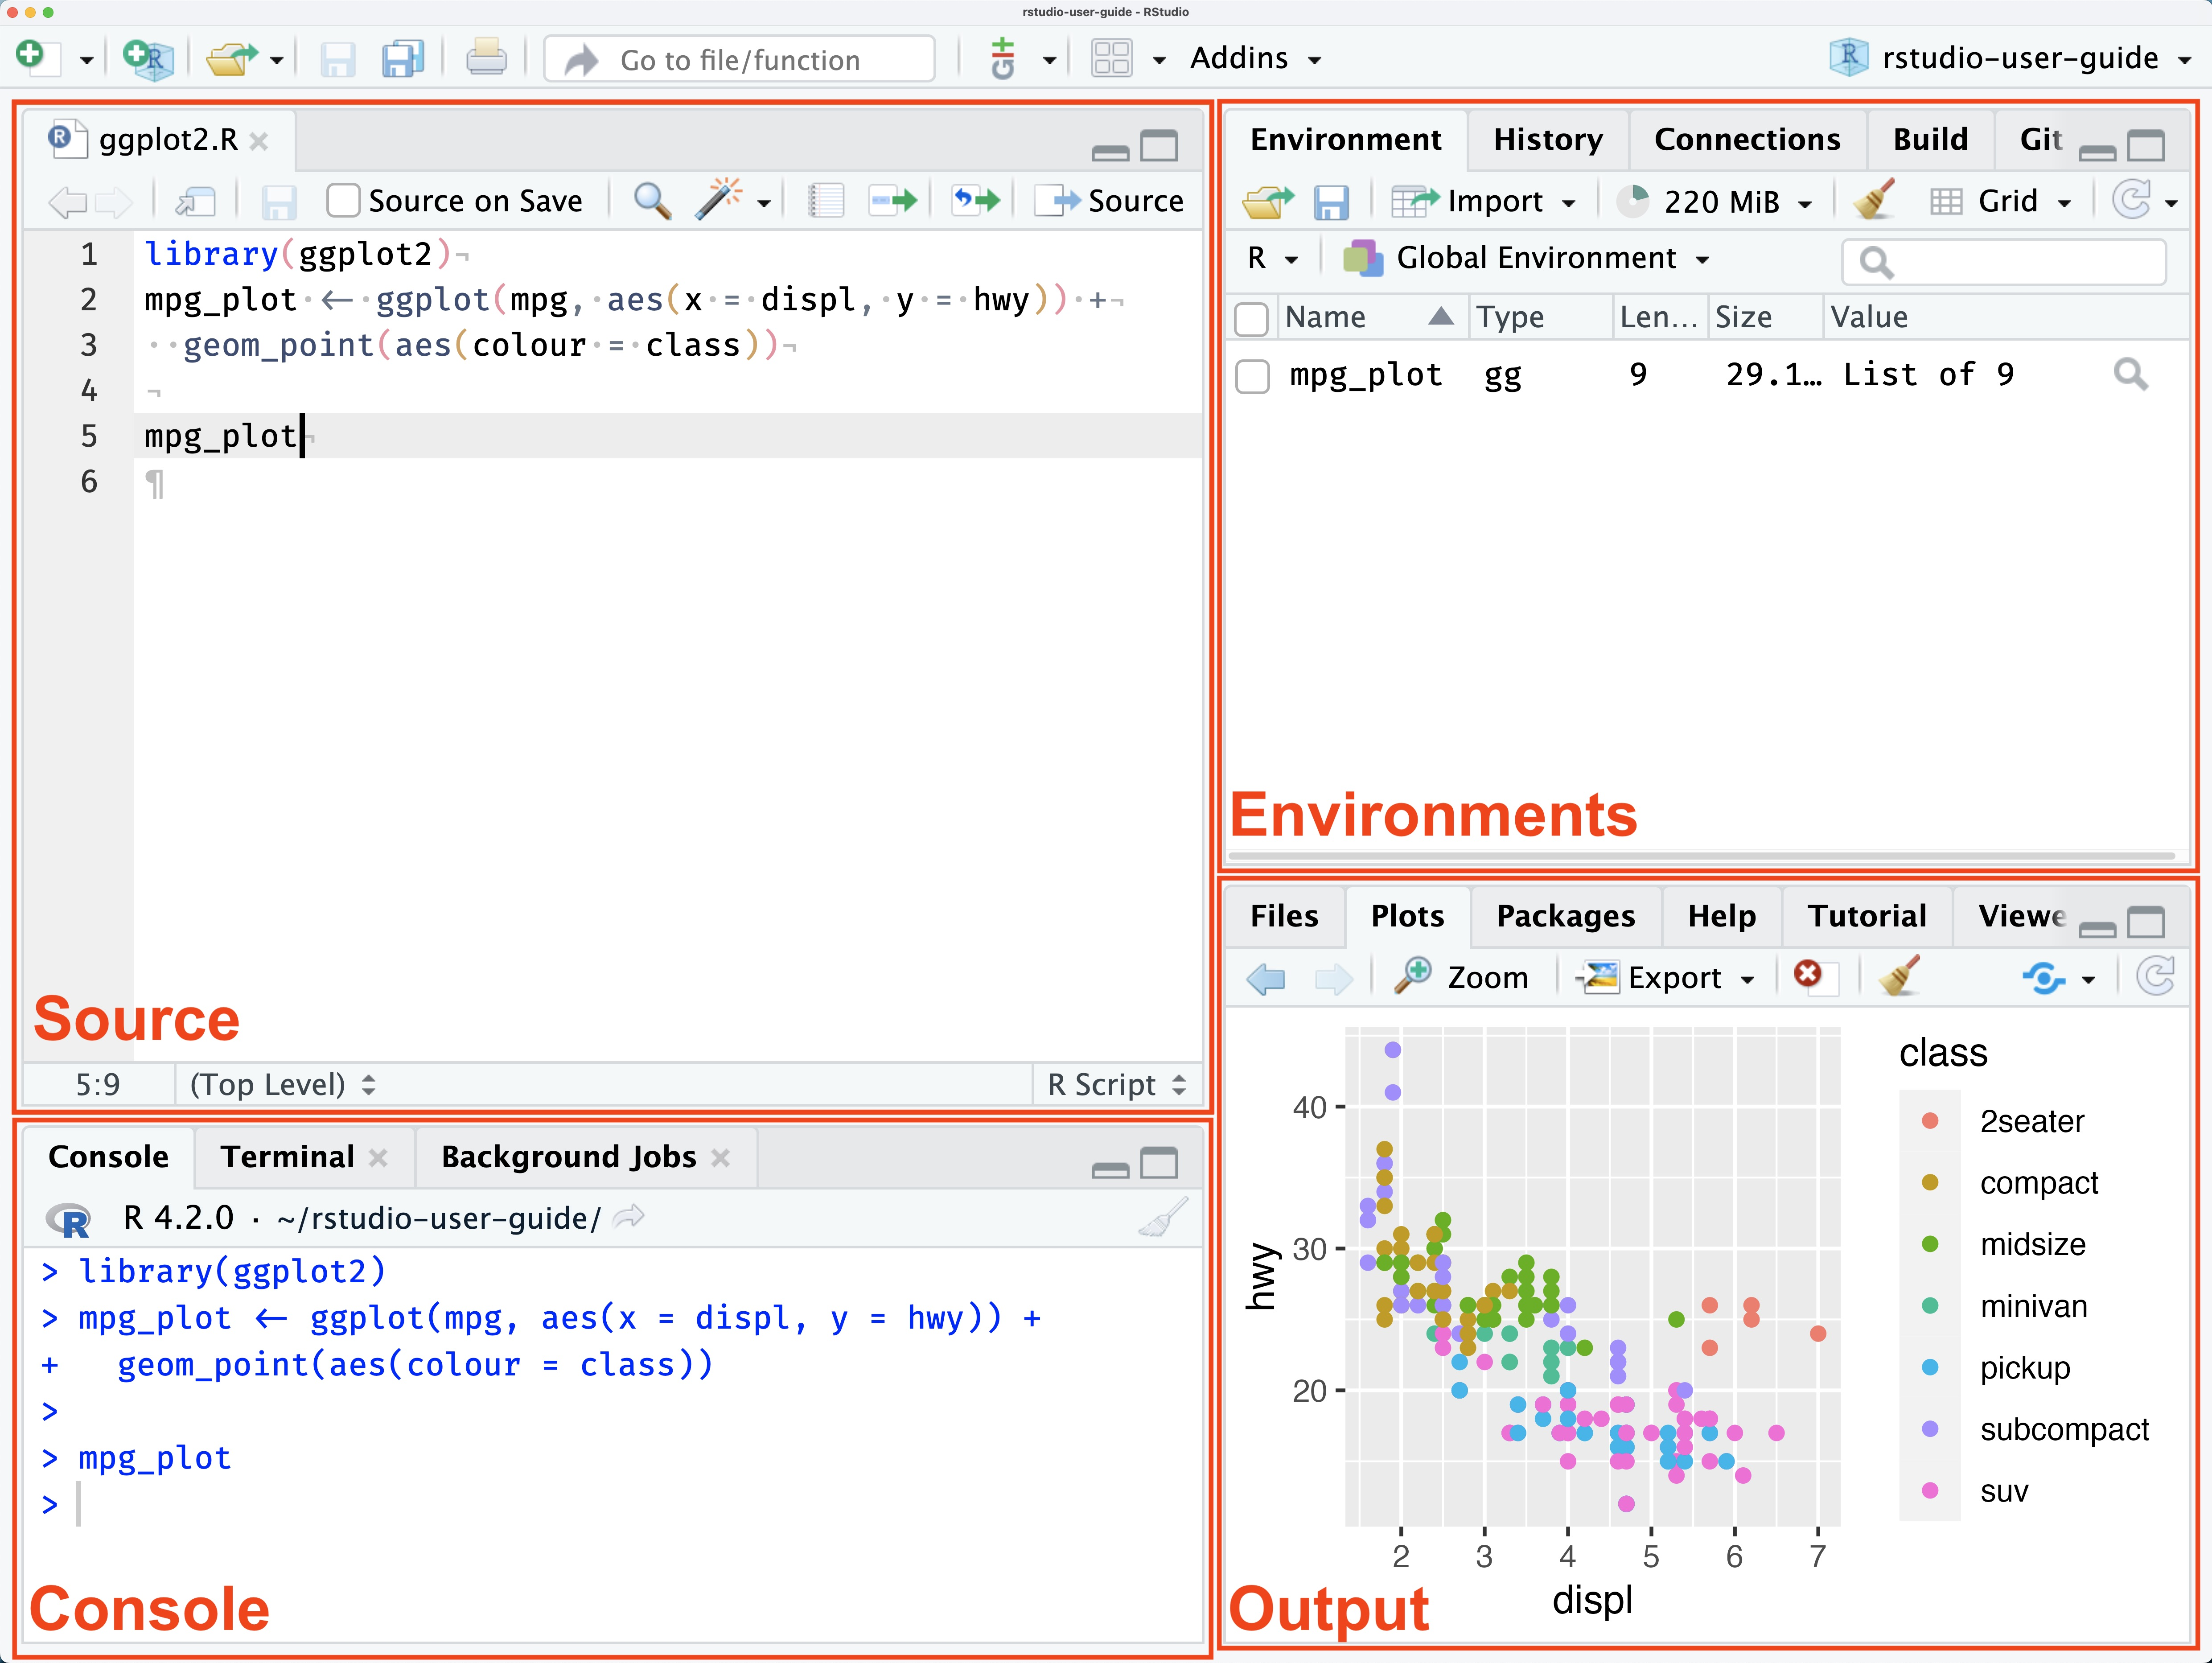
\includegraphics[width=5.125in,height=\textheight]{images/clipboard-2730531706.png}

}

\caption{Extraído de RStudio User Guide}

\end{figure}%

Hay cuatro paneles, cada uno indispensable y con un conjunto de
funcionalidades:

\begin{enumerate}
\def\labelenumi{\arabic{enumi}.}
\item
  \textbf{Source}: Todo el código que escribes en R se realiza en el
  panel Source. El código R es simplemente tu conjunto de instrucciones
  en el lenguaje R para que la computadora complete las tareas dadas.
\item
  \textbf{Consola}: La consola es la consola interactiva R. Aquí es
  donde la mayoría de las funciones se ejecutan al instante. Aquí es
  donde aparecen los resultados de los cálculos y procedimientos que
  hemos solicitado al programa. Se utiliza principalmente para una
  verificación rápida y también para ver el resultado de tus scripts.
\item
  \textbf{Entorno}: La pestaña Entorno es la lista de todos los objetos
  que has creado en tu trabajo. Algunos ejemplos de objetos son
  vectores, matrices, data frames, listas, gráficos y funciones.
\item
  \textbf{Archivos/Gráficos/Paquetes/Ayuda}:

  \begin{itemize}
  \tightlist
  \item
    \textbf{Archivos}: Son para navegar por el sistema de archivos de tu
    computadora directamente desde RStudio.
  \item
    \textbf{Gráficos}: Después de ejecutar el código R, puedes ver las
    imágenes creadas por el código R.
  \item
    \textbf{Paquetes}: La herramienta gestiona los paquetes que has
    instalado.
  \item
    \textbf{Ayuda}: El equivalente de Google para R. Puedes buscar
    cualquier información sobre las funciones e incluso encontrar el
    tutorial necesario.
  \end{itemize}
\end{enumerate}

La ventaja original del panel \textbf{Source} es la \textbf{capacidad de
editar rápidamente tu código}, el cual puedes volver a ejecutar. Este
aspecto incluye tanto la reproductividad como la eficiencia; por
ejemplo, podemos ajustar nuestro código sin rehacerlo desde cero.
Además, podemos guardar nuestro trabajo como un archivo, podemos
almacenar nuestros scripts en un editor de computadora, podemos
distribuirlo, podemos editarlo o publicar este archivo nuevamente. Pero
para trabajar de manera organizada, también es importante tener una
buena estructura para almacenar todo lo relacionado con el proyecto.

Cuando trabajamos en proyectos de análisis de datos, es común manejar
varios archivos relacionados: tus scripts (donde escribirás el código),
los datos que analizarás y los resultados generados. Tener una carpeta
específica para cada proyecto te ayuda a mantener todo organizado en un
solo lugar. Además, R necesita saber dónde buscar y guardar los
archivos, y eso se define mediante el~\textbf{directorio de trabajo},
que es simplemente la carpeta donde R guardará y buscará archivos
automáticamente para el proyecto en específico.

\section{Crear un archivo de script}\label{crear-un-archivo-de-script}

Cuando trabajamos en R, utilizamos diferentes tipos de archivos para
organizar y guardar nuestro trabajo. Dos formatos comunes son el
\textbf{archivo R Script} y el \textbf{documento Quarto}. Ambos se
utilizan para escribir código, pero cumplen propósitos diferentes que es
importante entender.

Un \textbf{archivo R Script} es un archivo simple donde escribimos y
guardamos nuestras instrucciones de código. Sirve como un registro de
los comandos que ejecutamos, permitiendo reutilizarlos o ajustarlos más
adelante. Sin embargo, este tipo de archivo no incluye espacio para
explicaciones extensas ni muestra los resultados directamente junto al
código.

En cambio, un \textbf{documento Quarto} va más allá al permitir combinar
texto explicativo, bloques de código y los resultados generados (como
tablas y gráficos) en un solo archivo. Además, es posible exportar el
archivo final en formatos como HTML, PDF o Word, haciéndolo ideal para
documentar y compartir análisis de manera profesional (de hecho, este
libro esta hecho en Quarto). Esta capacidad de integrar explicación,
análisis y presentación en un mismo lugar hace que Quarto sea
particularmente útil para aprender y comunicar análisis de datos. En
nuestras clases, vamos a utilizar \textbf{documentos Quarto}.

\begin{enumerate}
\def\labelenumi{\arabic{enumi}.}
\item
  \textbf{Accede a la ventana Files}:

  \begin{itemize}
  \tightlist
  \item
    En RStudio, localiza el panel \textbf{Files}. Este panel muestra el
    contenido de la carpeta de trabajo que configuraste previamente.
  \end{itemize}
\item
  \textbf{Crea un nuevo documento Quarto}:

  \begin{itemize}
  \tightlist
  \item
    En el panel \textbf{Files}, haz clic en el botón \textbf{New File} y
    selecciona \textbf{Quarto Document}.
  \end{itemize}

  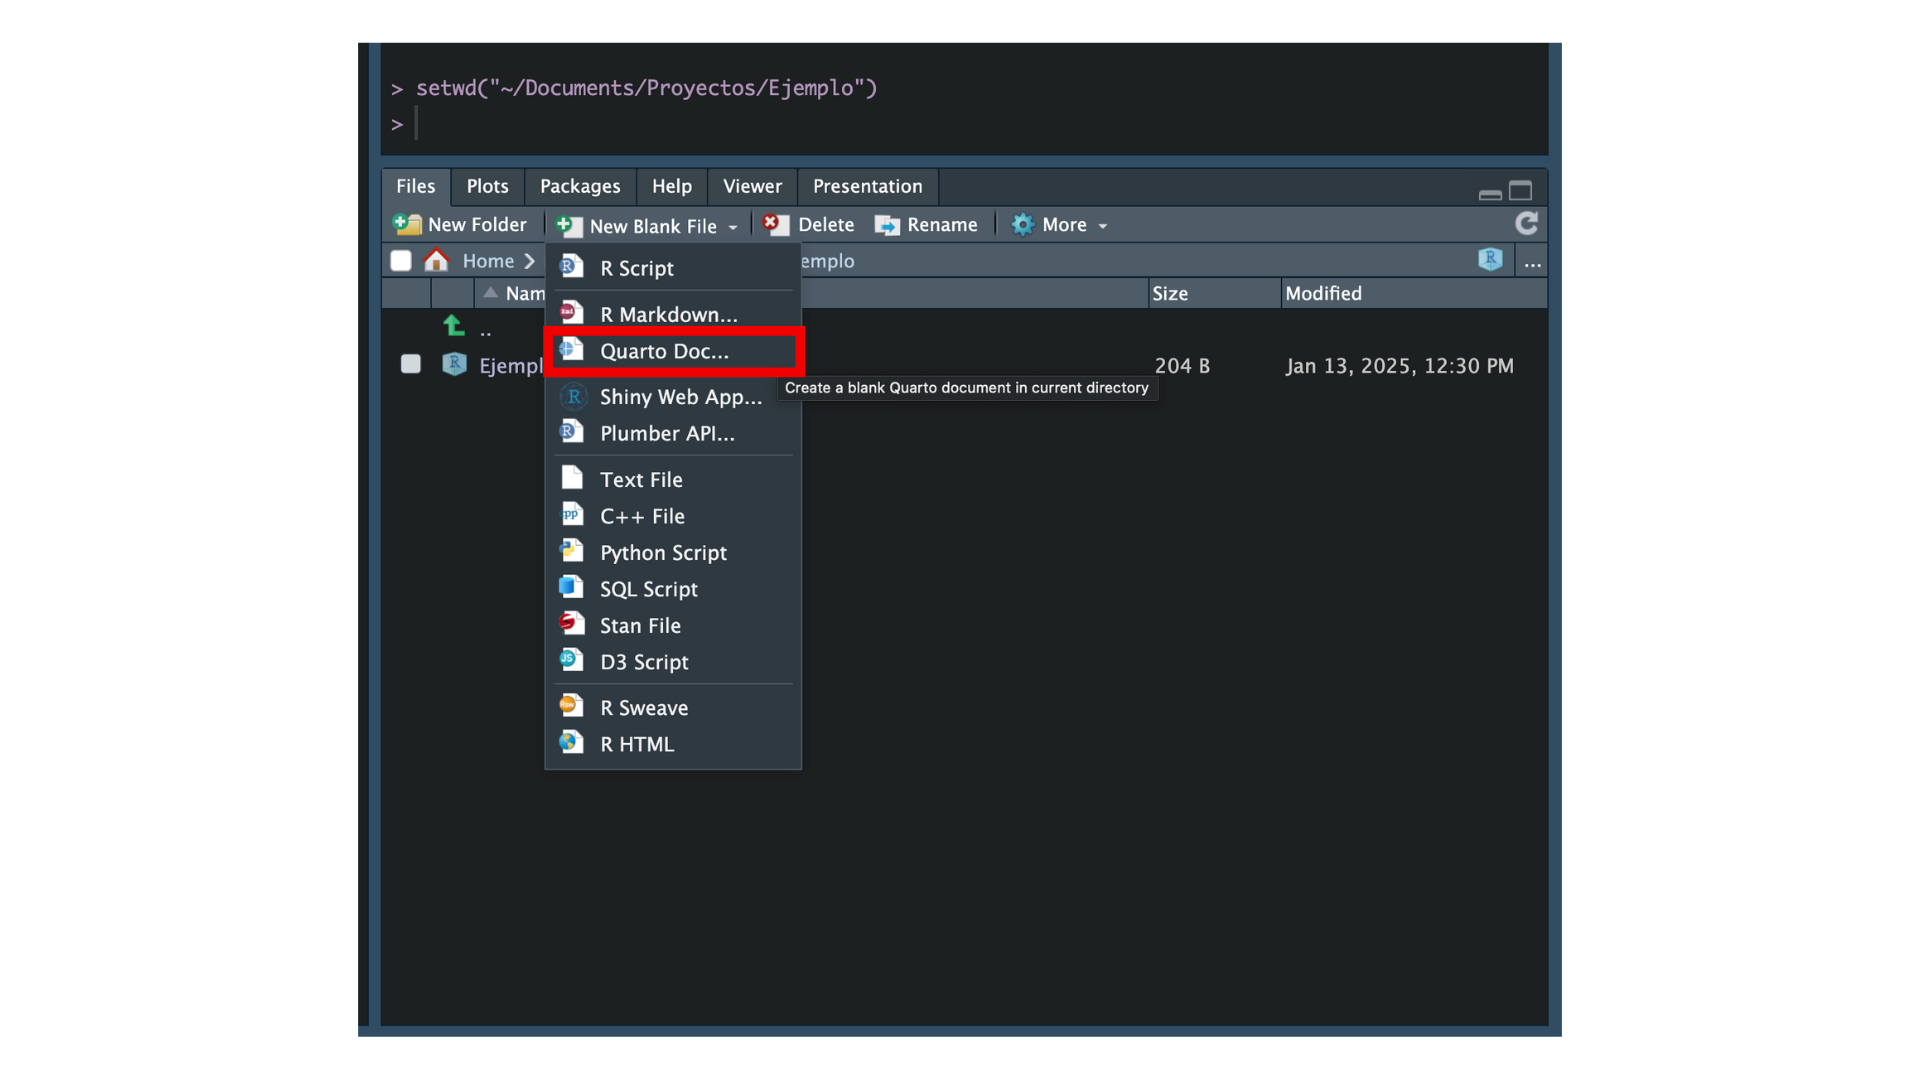
\includegraphics[width=6.72917in,height=\textheight]{images/9.png}

  \begin{itemize}
  \tightlist
  \item
    Aparecerá un cuadro de diálogo donde puedes configurar el título del
    documento, tu nombre y el formato de salida inicial (HTML es una
    buena opción para empezar). Haz clic en \textbf{Create}.
  \end{itemize}
\item
  \textbf{Guarda automáticamente en la carpeta de trabajo}:

  \begin{itemize}
  \tightlist
  \item
    Cuando crees el documento desde la ventana \textbf{Files}, este se
    guardará automáticamente en tu carpeta de trabajo configurada. No
    necesitas realizar pasos adicionales para seleccionar la ubicación.
  \end{itemize}
\end{enumerate}

En un archivo Quarto puedes combinar texto explicativo (en formato
Markdown) con bloques (chunks) de código en R. Los bloques de código son
las secciones donde escribirás las instrucciones que deseas ejecutar, y
están delimitados por tres backticks (```) seguidos del lenguaje que
estás utilizando (en este caso, \texttt{r}). Para agregar un bloque de
código de manera rápida, puedes utilizar el atajo de teclado:

\begin{itemize}
\tightlist
\item
  \textbf{Ctrl + Alt + I} en Windows y Linux.
\item
  \textbf{Cmd + Option + I} en Mac.
\end{itemize}

Este atajo insertará automáticamente un nuevo chunk en tu documento, con
la estructura básica para que puedas empezar a escribir tu código. Un
chunk de código tiene este formato:

\begin{Shaded}
\begin{Highlighting}[]
\CommentTok{\# Aquí escribes tu código en R}
\end{Highlighting}
\end{Shaded}

Dentro del chunk, puedes incluir cualquier instrucción que se ejecutará
cuando proceses el documento. Esto permite mantener el texto explicativo
y el código separados pero integrados en el mismo archivo.

\begin{tcolorbox}[enhanced jigsaw, titlerule=0mm, title=\textcolor{quarto-callout-important-color}{\faExclamation}\hspace{0.5em}{Importante}, colback=white, opacityback=0, breakable, toprule=.15mm, left=2mm, leftrule=.75mm, colframe=quarto-callout-important-color-frame, bottomtitle=1mm, rightrule=.15mm, opacitybacktitle=0.6, coltitle=black, arc=.35mm, bottomrule=.15mm, toptitle=1mm, colbacktitle=quarto-callout-important-color!10!white]

Es primordial que trabajes directamente desde tu carpeta de trabajo,
asegurando que todos los archivos relacionados con el proyecto estén
organizados en una carpeta.

\end{tcolorbox}

\chapter{Elementos}\label{elementos}

Los elementos son la unidad mínima de información. Puede representar un
valor numérico, una palabra, o una afirmación. Cuando usamos R,
escribimos estos elementos directamente en la consola o los usamos
dentro de otros objetos más grandes.

Saber reconocer qué tipo de elemento estamos usando es fundamental para
entender cómo se comporta en el código y qué operaciones podemos hacer
con él.

\begin{tcolorbox}[enhanced jigsaw, titlerule=0mm, title=\textcolor{quarto-callout-note-color}{\faInfo}\hspace{0.5em}{Dato}, colback=white, opacityback=0, breakable, toprule=.15mm, left=2mm, leftrule=.75mm, colframe=quarto-callout-note-color-frame, bottomtitle=1mm, rightrule=.15mm, opacitybacktitle=0.6, coltitle=black, arc=.35mm, bottomrule=.15mm, toptitle=1mm, colbacktitle=quarto-callout-note-color!10!white]

En R existen varios tipos de datos, pero podemos empezar por los tres
tipos básicos que se usan todo el tiempo:

\begin{itemize}
\item
  \textbf{Numéricos}, para representar cantidades.
\item
  \textbf{Texto}, para representar palabras o frases.
\item
  \textbf{Lógicos}, para representar afirmaciones verdaderas o falsas.
\end{itemize}

\end{tcolorbox}

Numérico

\begin{Shaded}
\begin{Highlighting}[]
\FunctionTok{class}\NormalTok{(}\DecValTok{5}\NormalTok{)}
\end{Highlighting}
\end{Shaded}

\begin{verbatim}
[1] "numeric"
\end{verbatim}

\begin{Shaded}
\begin{Highlighting}[]
\SpecialCharTok{{-}}\DecValTok{3}
\end{Highlighting}
\end{Shaded}

\begin{verbatim}
[1] -3
\end{verbatim}

\begin{Shaded}
\begin{Highlighting}[]
\FloatTok{3.5}
\end{Highlighting}
\end{Shaded}

\begin{verbatim}
[1] 3.5
\end{verbatim}

Texto

\begin{Shaded}
\begin{Highlighting}[]
\FunctionTok{class}\NormalTok{(}\StringTok{"Hola"}\NormalTok{)}
\end{Highlighting}
\end{Shaded}

\begin{verbatim}
[1] "character"
\end{verbatim}

\begin{Shaded}
\begin{Highlighting}[]
\StringTok{"Perú"}
\end{Highlighting}
\end{Shaded}

\begin{verbatim}
[1] "Perú"
\end{verbatim}

\begin{Shaded}
\begin{Highlighting}[]
\StringTok{"El servicio fue ineficiente"}
\end{Highlighting}
\end{Shaded}

\begin{verbatim}
[1] "El servicio fue ineficiente"
\end{verbatim}

Lógico (verdadero/falso)

\begin{Shaded}
\begin{Highlighting}[]
\FunctionTok{class}\NormalTok{(T)}
\end{Highlighting}
\end{Shaded}

\begin{verbatim}
[1] "logical"
\end{verbatim}

\begin{Shaded}
\begin{Highlighting}[]
\NormalTok{F}
\end{Highlighting}
\end{Shaded}

\begin{verbatim}
[1] FALSE
\end{verbatim}

\section{Operaciones básicas con
elementos}\label{operaciones-buxe1sicas-con-elementos}

En R, al igual que en otros lenguajes de programación, es fundamental
comprender cómo manipular distintos tipos de datos mediante operaciones
básicas.

\subsection{Operadores matemáticos:}\label{operadores-matemuxe1ticos}

Permiten realizar cálculos aritméticos entre valores.

\begin{itemize}
\tightlist
\item
  \(a + b\) → \texttt{a\ +\ b}\\
\item
  \(a - b\) → \texttt{a\ -\ b}\\
\item
  \(a \times b\) → \texttt{a\ *\ b}\\
\item
  \(\frac{a}{b}\) → \texttt{a\ /\ b}\\
\item
  \(a^b\) → \texttt{a\ \^{}\ b}\\
\item
  \(\sqrt{a}\) → \texttt{sqrt(a)}
\end{itemize}

Suma

\begin{Shaded}
\begin{Highlighting}[]
\DecValTok{5} \SpecialCharTok{+} \DecValTok{3}
\end{Highlighting}
\end{Shaded}

\begin{verbatim}
[1] 8
\end{verbatim}

Resta

\begin{Shaded}
\begin{Highlighting}[]
\DecValTok{10} \SpecialCharTok{{-}} \DecValTok{4}
\end{Highlighting}
\end{Shaded}

\begin{verbatim}
[1] 6
\end{verbatim}

Multiplicación

\begin{Shaded}
\begin{Highlighting}[]
\DecValTok{5}\SpecialCharTok{*}\DecValTok{6}
\end{Highlighting}
\end{Shaded}

\begin{verbatim}
[1] 30
\end{verbatim}

División

\begin{Shaded}
\begin{Highlighting}[]
\DecValTok{30}\SpecialCharTok{/}\DecValTok{5}
\end{Highlighting}
\end{Shaded}

\begin{verbatim}
[1] 6
\end{verbatim}

Potencia:

\begin{Shaded}
\begin{Highlighting}[]
\DecValTok{5}\SpecialCharTok{\^{}}\DecValTok{2}
\end{Highlighting}
\end{Shaded}

\begin{verbatim}
[1] 25
\end{verbatim}

Operaciones en paréntesis

\begin{Shaded}
\begin{Highlighting}[]
\NormalTok{(}\DecValTok{2} \SpecialCharTok{+} \DecValTok{3}\NormalTok{) }\SpecialCharTok{*} \DecValTok{10} 
\end{Highlighting}
\end{Shaded}

\begin{verbatim}
[1] 50
\end{verbatim}

Los elementos lógicos son tratados como 0 y 1

\begin{Shaded}
\begin{Highlighting}[]
\ConstantTok{FALSE} \SpecialCharTok{+} \ConstantTok{FALSE}
\end{Highlighting}
\end{Shaded}

\begin{verbatim}
[1] 0
\end{verbatim}

\begin{Shaded}
\begin{Highlighting}[]
\ConstantTok{TRUE} \SpecialCharTok{+} \ConstantTok{TRUE}
\end{Highlighting}
\end{Shaded}

\begin{verbatim}
[1] 2
\end{verbatim}

\begin{Shaded}
\begin{Highlighting}[]
\ConstantTok{TRUE} \SpecialCharTok{+} \ConstantTok{FALSE}
\end{Highlighting}
\end{Shaded}

\begin{verbatim}
[1] 1
\end{verbatim}

\begin{tcolorbox}[enhanced jigsaw, titlerule=0mm, title=\textcolor{quarto-callout-caution-color}{\faFire}\hspace{0.5em}{Cuidado}, colback=white, opacityback=0, breakable, toprule=.15mm, left=2mm, leftrule=.75mm, colframe=quarto-callout-caution-color-frame, bottomtitle=1mm, rightrule=.15mm, opacitybacktitle=0.6, coltitle=black, arc=.35mm, bottomrule=.15mm, toptitle=1mm, colbacktitle=quarto-callout-caution-color!10!white]

Los \textbf{elementos de texto} no están diseñados para realizar
operaciones aritméticas como suma o multiplicación. Si intentas hacerlo,
obtendrás un error. Esto se debe a que, a diferencia de los números, el
texto no representa cantidades numéricas sobre las que se pueda operar.

\end{tcolorbox}

Error:

\begin{verbatim}
"Hola" + "Que tal"
\end{verbatim}

Error in ``Hola'' + ``Que tal'' : non-numeric argument to binary
operator

\subsection{Operadores de
comparación}\label{operadores-de-comparaciuxf3n}

Permiten evaluar relaciones entre valores. Devuelven siempre un valor
lógico: \texttt{TRUE} o \texttt{FALSE}.

\begin{itemize}
\tightlist
\item
  \(x = y\) → \texttt{x\ ==\ y}: Igualdad
\item
  \(x \neq y\) → \texttt{x\ !=\ y}: Desigualdad
\item
  \(x < y\): Menor que
\item
  \(x \leq y\) → \texttt{x\ \textless{}=\ y}: Menor o igual que
\item
  \(x > y\): Mayor que
\item
  \(x \geq y\) → \texttt{x\ \textgreater{}=\ y}: Mayor o igual que
\end{itemize}

\begin{Shaded}
\begin{Highlighting}[]
\DecValTok{5} \SpecialCharTok{==} \DecValTok{5}   
\end{Highlighting}
\end{Shaded}

\begin{verbatim}
[1] TRUE
\end{verbatim}

\begin{Shaded}
\begin{Highlighting}[]
\DecValTok{3} \SpecialCharTok{!=} \DecValTok{2}    
\end{Highlighting}
\end{Shaded}

\begin{verbatim}
[1] TRUE
\end{verbatim}

\begin{Shaded}
\begin{Highlighting}[]
\DecValTok{10} \SpecialCharTok{\textless{}} \DecValTok{8}    
\end{Highlighting}
\end{Shaded}

\begin{verbatim}
[1] FALSE
\end{verbatim}

\begin{Shaded}
\begin{Highlighting}[]
\DecValTok{4} \SpecialCharTok{\textgreater{}=} \DecValTok{4}     
\end{Highlighting}
\end{Shaded}

\begin{verbatim}
[1] TRUE
\end{verbatim}

\subsection{Operadores lógicos}\label{operadores-luxf3gicos}

Permiten combinar condiciones. Estas expresiones también devuelven
\texttt{TRUE} o \texttt{FALSE}.

\begin{itemize}
\item
  \textbf{Negación lógica}: \(\lnot x\) → \texttt{!x} Invierte el valor
  lógico de \texttt{x}.
\item
  \textbf{Conjunción lógica (Y)}: \(x \land y\) → \texttt{x\ \&\ y}
  Devuelve \texttt{TRUE} solo si \textbf{ambas} condiciones son
  verdaderas.
\item
  \textbf{Disyunción lógica (O)}: \(x \lor y\) →
  \texttt{x\ \textbar{}\ y} Devuelve \texttt{TRUE} si \textbf{al menos
  una} condición es verdadera.
\end{itemize}

\textbf{Negación lógica}

\begin{Shaded}
\begin{Highlighting}[]
\SpecialCharTok{!}\ConstantTok{TRUE}    
\end{Highlighting}
\end{Shaded}

\begin{verbatim}
[1] FALSE
\end{verbatim}

\begin{Shaded}
\begin{Highlighting}[]
\SpecialCharTok{!}\ConstantTok{FALSE}    
\end{Highlighting}
\end{Shaded}

\begin{verbatim}
[1] TRUE
\end{verbatim}

\textbf{Conjunción lógica (Y)}

\begin{Shaded}
\begin{Highlighting}[]
\NormalTok{  (}\DecValTok{5} \SpecialCharTok{\textgreater{}} \DecValTok{3}\NormalTok{) }\SpecialCharTok{\&}\NormalTok{ (}\DecValTok{2} \SpecialCharTok{\textless{}} \DecValTok{4}\NormalTok{)   }
\end{Highlighting}
\end{Shaded}

\begin{verbatim}
[1] TRUE
\end{verbatim}

\begin{Shaded}
\begin{Highlighting}[]
\NormalTok{  (}\DecValTok{10} \SpecialCharTok{\textgreater{}} \DecValTok{3}\NormalTok{) }\SpecialCharTok{\&}\NormalTok{ (}\DecValTok{1} \SpecialCharTok{\textgreater{}} \DecValTok{5}\NormalTok{)  }
\end{Highlighting}
\end{Shaded}

\begin{verbatim}
[1] FALSE
\end{verbatim}

\textbf{Disyunción lógica (O)}:

\begin{Shaded}
\begin{Highlighting}[]
\NormalTok{  (}\DecValTok{4} \SpecialCharTok{\textless{}} \DecValTok{2}\NormalTok{) }\SpecialCharTok{|}\NormalTok{ (}\DecValTok{7} \SpecialCharTok{\textgreater{}} \DecValTok{1}\NormalTok{)   }
\end{Highlighting}
\end{Shaded}

\begin{verbatim}
[1] TRUE
\end{verbatim}

\begin{Shaded}
\begin{Highlighting}[]
\NormalTok{  (}\DecValTok{3} \SpecialCharTok{==} \DecValTok{5}\NormalTok{) }\SpecialCharTok{|}\NormalTok{ (}\DecValTok{2} \SpecialCharTok{\textgreater{}} \DecValTok{10}\NormalTok{) }
\end{Highlighting}
\end{Shaded}

\begin{verbatim}
[1] FALSE
\end{verbatim}

\chapter{Objetos}\label{objetos}

Los objetos son estructuras donde guardamos información para poder
reutilizarla, manipularla o transformarla más adelante.

Crear un objeto es como ponerle nombre a un dato o conjunto de datos.
Una vez creado, ese nombre puede usarse para hacer cálculos, funciones,
gráficos y más.

\begin{tcolorbox}[enhanced jigsaw, titlerule=0mm, title=\textcolor{quarto-callout-note-color}{\faInfo}\hspace{0.5em}{Dato}, colback=white, opacityback=0, breakable, toprule=.15mm, left=2mm, leftrule=.75mm, colframe=quarto-callout-note-color-frame, bottomtitle=1mm, rightrule=.15mm, opacitybacktitle=0.6, coltitle=black, arc=.35mm, bottomrule=.15mm, toptitle=1mm, colbacktitle=quarto-callout-note-color!10!white]

En R, los objetos se crean con el operador \texttt{\textless{}-} o el
\texttt{=}, que se lee como ``le asigno''.

Por ejemplo:

\begin{Shaded}
\begin{Highlighting}[]
\NormalTok{x }\OtherTok{=} \DecValTok{5}
\end{Highlighting}
\end{Shaded}

Aquí estamos diciendo: crea un objeto llamado x y asígnale el número 5.

\end{tcolorbox}

\textbf{¿Qué puedo guardar en un objeto?}

Prácticamente todo, puedes guardar:

\begin{itemize}
\tightlist
\item
  Un número: \texttt{x\ =\ 10}
\item
  Una palabra: \texttt{nombre\ =\ "Gonzalo"}
\item
  Un valor lógico: \texttt{es\_mayor\ =\ TRUE}
\end{itemize}

Una vez creado el objeto, puedes \textbf{llamarlo por su nombre}:

Si

\begin{Shaded}
\begin{Highlighting}[]
\NormalTok{x }\OtherTok{=} \DecValTok{10}
\end{Highlighting}
\end{Shaded}

Entonces\ldots{}

\begin{Shaded}
\begin{Highlighting}[]
\NormalTok{x}
\end{Highlighting}
\end{Shaded}

\begin{verbatim}
[1] 10
\end{verbatim}

Y también \textbf{usarlo en operaciones}:

Siendo \(x = 10\)\ldots{}

\begin{Shaded}
\begin{Highlighting}[]
\NormalTok{x }\SpecialCharTok{+} \DecValTok{2}
\end{Highlighting}
\end{Shaded}

\begin{verbatim}
[1] 12
\end{verbatim}

\begin{tcolorbox}[enhanced jigsaw, titlerule=0mm, title=\textcolor{quarto-callout-tip-color}{\faLightbulb}\hspace{0.5em}{Consejo}, colback=white, opacityback=0, breakable, toprule=.15mm, left=2mm, leftrule=.75mm, colframe=quarto-callout-tip-color-frame, bottomtitle=1mm, rightrule=.15mm, opacitybacktitle=0.6, coltitle=black, arc=.35mm, bottomrule=.15mm, toptitle=1mm, colbacktitle=quarto-callout-tip-color!10!white]

Un buen nombre para un objeto debe ser claro, sin espacios ni tildes.
Puedes usar guiones bajos (\_) para separar palabras: por ejemplo,
\texttt{edad\_promedio} es mucho mejor que \texttt{ep} o \texttt{e.p.}.

\end{tcolorbox}

\section{Tipos de objetos en R}\label{tipos-de-objetos-en-r}

En R, no todo es solo un número o una palabra. Muchas veces necesitamos
guardar varios elementos juntos, y para eso usamos diferentes tipos de
objetos. Cada uno tiene su propia estructura y sirve para distintos
propósitos.

\subsection{Los principales tipos de objetos
son:}\label{los-principales-tipos-de-objetos-son}

\textbf{Vectores}

Conjunto de elementos del \emph{mismo tipo} (todos números, o todos
textos, o todos lógicos).

\begin{Shaded}
\begin{Highlighting}[]
\NormalTok{edades }\OtherTok{=} \FunctionTok{c}\NormalTok{(}\DecValTok{18}\NormalTok{, }\DecValTok{21}\NormalTok{, }\DecValTok{25}\NormalTok{)}
\NormalTok{nombres }\OtherTok{=} \FunctionTok{c}\NormalTok{(}\StringTok{"Ana"}\NormalTok{, }\StringTok{"Luis"}\NormalTok{, }\StringTok{"María"}\NormalTok{)}
\end{Highlighting}
\end{Shaded}

\begin{Shaded}
\begin{Highlighting}[]
\NormalTok{edades}
\end{Highlighting}
\end{Shaded}

\begin{verbatim}
[1] 18 21 25
\end{verbatim}

\begin{Shaded}
\begin{Highlighting}[]
\NormalTok{nombres}
\end{Highlighting}
\end{Shaded}

\begin{verbatim}
[1] "Ana"   "Luis"  "María"
\end{verbatim}

\textbf{Matrices}

Como una tabla, pero con \textbf{solo un tipo de dato} (por ejemplo,
solo números).

\begin{Shaded}
\begin{Highlighting}[]
\NormalTok{matriz }\OtherTok{=} \FunctionTok{matrix}\NormalTok{(}\DecValTok{1}\SpecialCharTok{:}\DecValTok{6}\NormalTok{, }\AttributeTok{nrow =} \DecValTok{2}\NormalTok{)}
\end{Highlighting}
\end{Shaded}

\begin{Shaded}
\begin{Highlighting}[]
\NormalTok{matriz}
\end{Highlighting}
\end{Shaded}

\begin{verbatim}
     [,1] [,2] [,3]
[1,]    1    3    5
[2,]    2    4    6
\end{verbatim}

\textbf{Listas}

Conjunto de elementos que \textbf{pueden ser de distintos tipos y
formas}.

\begin{Shaded}
\begin{Highlighting}[]
\NormalTok{mi\_lista }\OtherTok{=} \FunctionTok{list}\NormalTok{(}\AttributeTok{nombre =} \StringTok{"Andrés"}\NormalTok{, edades, }\AttributeTok{aprobado =} \ConstantTok{TRUE}\NormalTok{)}
\end{Highlighting}
\end{Shaded}

\begin{Shaded}
\begin{Highlighting}[]
\NormalTok{mi\_lista}
\end{Highlighting}
\end{Shaded}

\begin{verbatim}
$nombre
[1] "Andrés"

[[2]]
[1] 18 21 25

$aprobado
[1] TRUE
\end{verbatim}

\textbf{Data frames}

La estructura más usada para bases de datos. Cada columna es un vector y
puede tener un tipo diferente (números, textos, etc.).

\begin{Shaded}
\begin{Highlighting}[]
\NormalTok{datos }\OtherTok{=} \FunctionTok{data.frame}\NormalTok{(}\AttributeTok{nombre =} \FunctionTok{c}\NormalTok{(}\StringTok{"Ana"}\NormalTok{, }\StringTok{"Luis"}\NormalTok{), }\AttributeTok{edad =} \FunctionTok{c}\NormalTok{(}\DecValTok{18}\NormalTok{, }\DecValTok{21}\NormalTok{),}
                   \AttributeTok{aprobado =} \FunctionTok{c}\NormalTok{(T, F), }\AttributeTok{horas\_estudio =} \FunctionTok{c}\NormalTok{(}\DecValTok{15}\NormalTok{, }\DecValTok{9}\NormalTok{))}
\end{Highlighting}
\end{Shaded}

\begin{Shaded}
\begin{Highlighting}[]
\NormalTok{datos}
\end{Highlighting}
\end{Shaded}

\begin{verbatim}
  nombre edad aprobado horas_estudio
1    Ana   18     TRUE            15
2   Luis   21    FALSE             9
\end{verbatim}

Al trabajar con datos en R, no solo importa tener la información:
también importa cómo está organizada. Los objetos nos permiten guardar,
transformar y analizar datos de formas muy distintas. Por eso, conocer
sus tipos es esencial.

\begin{tcolorbox}[enhanced jigsaw, titlerule=0mm, title=\textcolor{quarto-callout-note-color}{\faInfo}\hspace{0.5em}{Dato}, colback=white, opacityback=0, breakable, toprule=.15mm, left=2mm, leftrule=.75mm, colframe=quarto-callout-note-color-frame, bottomtitle=1mm, rightrule=.15mm, opacitybacktitle=0.6, coltitle=black, arc=.35mm, bottomrule=.15mm, toptitle=1mm, colbacktitle=quarto-callout-note-color!10!white]

Cada tipo de objeto cumple un rol distinto:

\begin{itemize}
\item
  Un \textbf{vector} te permite guardar variables como edad, ingresos o
  respuestas a una encuesta.
\item
  Un \textbf{data frame} organiza esas variables como columnas, ideal
  para trabajar con bases de datos reales.
\item
  Una \textbf{lista} puede guardar resultados de modelos, gráficos o
  varios tipos de objetos juntos.
\end{itemize}

\end{tcolorbox}

\chapter{Funciones}\label{funciones}

Hasta ahora hemos usado expresiones como \texttt{c()},
\texttt{matrix()}, \texttt{list()} o \texttt{data.frame()} para crear
objetos. Todas estas expresiones tienen algo en común: \textbf{son
funciones}.

Una función en R es una herramienta que realiza una tarea específica.
Tiene un nombre (como \texttt{sum()} o \texttt{mean()}), y entre
paréntesis le damos la información que necesita para trabajar: estos son
los \textbf{argumentos} de la función.

Piensa en la funciones como pequeñas máquinas: tú pones algo dentro, la
función lo procesa y te devuelve un resultado.

\begin{figure}[H]

{\centering 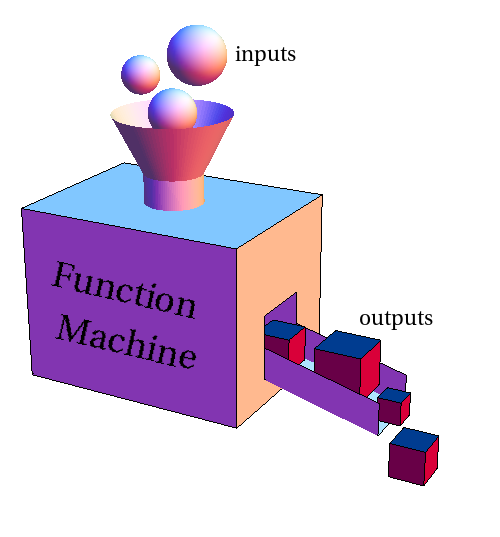
\includegraphics[width=5.05208in,height=\textheight]{images/clipboard-1257493817.png}

}

\caption{Extraído de: https://mathinsight.org/function\_machine}

\end{figure}%

En R \textbf{todo se hace con funciones}: importar datos, limpiar
variables, calcular estadísticas, hacer gráficos o modelos,todo eso se
logra llamando a funciones específicas.

Saber cómo usar una función y cómo entender lo que devuelve, es uno de
los pasos más importantes para poder avanzar en análisis de datos con R.
\textbf{Por ejemplo:}

\texttt{c()}: Esta función \textbf{combina elementos} para volverlos
vectores. Si le das \texttt{1}, \texttt{2} y \texttt{3}, te devuelve un
solo objeto que los contiene:

\begin{Shaded}
\begin{Highlighting}[]
\FunctionTok{c}\NormalTok{(}\DecValTok{1}\NormalTok{, }\DecValTok{2}\NormalTok{, }\DecValTok{3}\NormalTok{) }
\end{Highlighting}
\end{Shaded}

\begin{verbatim}
[1] 1 2 3
\end{verbatim}

\texttt{sum()}: Esta función \textbf{suma} los números que le das. Si
metes \texttt{5}, \texttt{10} y \texttt{15}, te devuelve \texttt{30}:

\begin{Shaded}
\begin{Highlighting}[]
\FunctionTok{sum}\NormalTok{(}\DecValTok{5}\NormalTok{, }\DecValTok{10}\NormalTok{, }\DecValTok{15}\NormalTok{)  }
\end{Highlighting}
\end{Shaded}

\begin{verbatim}
[1] 30
\end{verbatim}

Algunas funciones permiten no solo darles valores, sino también ajustar
cómo se comportan usando otros argumentos. Por ejemplo, la función
mean() puede recibir instrucciones adicionales como trim o na.rm.

\begin{tcolorbox}[enhanced jigsaw, titlerule=0mm, title=\textcolor{quarto-callout-tip-color}{\faLightbulb}\hspace{0.5em}{Consejo}, colback=white, opacityback=0, breakable, toprule=.15mm, left=2mm, leftrule=.75mm, colframe=quarto-callout-tip-color-frame, bottomtitle=1mm, rightrule=.15mm, opacitybacktitle=0.6, coltitle=black, arc=.35mm, bottomrule=.15mm, toptitle=1mm, colbacktitle=quarto-callout-tip-color!10!white]

Cuando una función necesita varios valores como insumo (por ejemplo,
varios números), estos deben ir agrupados dentro de un vector, usando
\texttt{c()}. Así, le estás dando a la función un solo bloque de datos,
y evita confsuión con otros argumentos.

\end{tcolorbox}

\texttt{mean()}: Esta función \textbf{calcula la media aritmética} de
los valores que pongas dentro:

\begin{Shaded}
\begin{Highlighting}[]
\FunctionTok{mean}\NormalTok{(}\FunctionTok{c}\NormalTok{(}\DecValTok{10}\NormalTok{, }\DecValTok{20}\NormalTok{, }\DecValTok{30}\NormalTok{)) }
\end{Highlighting}
\end{Shaded}

\begin{verbatim}
[1] 20
\end{verbatim}

Aunque parezca que solo le estamos pasando tres números, en realidad
estamos entregándole \textbf{un solo objeto}: un \textbf{vector} que
contiene esos valores.

Pero también podemos darle más indicaciones a través de otros argumentos

Este promedio elimina los datos faltantes (NA) antes de hacer el
cálculo:

\begin{Shaded}
\begin{Highlighting}[]
\FunctionTok{mean}\NormalTok{(}\FunctionTok{c}\NormalTok{(}\DecValTok{10}\NormalTok{, }\DecValTok{20}\NormalTok{, }\ConstantTok{NA}\NormalTok{, }\DecValTok{30}\NormalTok{), }\AttributeTok{na.rm =} \ConstantTok{TRUE}\NormalTok{)}
\end{Highlighting}
\end{Shaded}

\begin{verbatim}
[1] 20
\end{verbatim}

Aquí calculamos el promedio después de eliminar un 20\% de los valores
extremos (en total, un 10\% abajo y un 10\% arriba). Esto es útil cuando
hay valores atípicos que podrían distorsionar el promedio.

\begin{Shaded}
\begin{Highlighting}[]
\FunctionTok{mean}\NormalTok{(}\FunctionTok{c}\NormalTok{(}\FloatTok{0.5}\NormalTok{, }\DecValTok{20}\NormalTok{, }\DecValTok{30}\NormalTok{, }\DecValTok{40}\NormalTok{, }\DecValTok{100}\NormalTok{), }\AttributeTok{trim =} \FloatTok{0.2}\NormalTok{)}
\end{Highlighting}
\end{Shaded}

\begin{verbatim}
[1] 30
\end{verbatim}

Así como puedes darle un bloque de datos a una función, también puedes
pedirle que \textbf{cuente cuántos elementos hay en un detemrinado
objeto}. Para eso usamos la función \texttt{length()}.

\begin{Shaded}
\begin{Highlighting}[]
\FunctionTok{length}\NormalTok{(}\FunctionTok{c}\NormalTok{(}\DecValTok{5}\NormalTok{, }\DecValTok{8}\NormalTok{, }\DecValTok{10}\NormalTok{))}
\end{Highlighting}
\end{Shaded}

\begin{verbatim}
[1] 3
\end{verbatim}

Este código le pide a R que diga cuántos elementos hay dentro del
vector. En este caso, la respuesta será \texttt{3} porque el vector
tiene tres números.

\texttt{length()} no se limita a vectores numéricos. También puedes
usarlo con vectores de texto, lógicos, o listas. Es una función muy útil
para \textbf{entender el tamaño de un objeto}, especialmente cuando
estás explorando o limpiando datos.

\begin{Shaded}
\begin{Highlighting}[]
\FunctionTok{length}\NormalTok{(}\FunctionTok{c}\NormalTok{(}\StringTok{"perro"}\NormalTok{, }\StringTok{"gato"}\NormalTok{, }\StringTok{"ratón"}\NormalTok{))}
\end{Highlighting}
\end{Shaded}

\begin{verbatim}
[1] 3
\end{verbatim}

\begin{tcolorbox}[enhanced jigsaw, titlerule=0mm, title=\textcolor{quarto-callout-tip-color}{\faLightbulb}\hspace{0.5em}{A tomar en cuenta}, colback=white, opacityback=0, breakable, toprule=.15mm, left=2mm, leftrule=.75mm, colframe=quarto-callout-tip-color-frame, bottomtitle=1mm, rightrule=.15mm, opacitybacktitle=0.6, coltitle=black, arc=.35mm, bottomrule=.15mm, toptitle=1mm, colbacktitle=quarto-callout-tip-color!10!white]

El análisis de datos se construye \textbf{función por función}. Cada
paso, desde importar los datos hasta graficarlos, implica aplicar una
función distinta. Aquí algunos ejemplos:

\begin{itemize}
\tightlist
\item
  \texttt{read.csv("datos.csv")} → \textbf{Leer datos} desde un archivo
  \texttt{.csv}.
\item
  \texttt{mean(ingresos)} → \textbf{Calcular el promedio} de una
  variable numérica.
\item
  \texttt{table(sexo)} → \textbf{Contar frecuencias} de una variable
  categórica.
\item
  \texttt{plot(edad,\ ingresos)} → \textbf{Graficar} la relación entre
  dos variables.
\item
  \texttt{summary(datos)} → \textbf{Resumir} un conjunto de datos.
\end{itemize}

\end{tcolorbox}

\textbf{Aprender funciones en R es como aprender vocabulario en un
idioma}: cada función es como una palabra con un uso y una forma
particular. Algunas hacen algo con lo que les das (como
\texttt{mean()}), otras simplemente te devuelven información (como
\texttt{length()}). Saber cómo se usan es lo que te permite construir
sentencias útiles en lenguaje R.

\chapter{Data Frames}\label{data-frames}

Cuando recolectamos o hacemos uso de conjuntos de datos, estos suelen
estar almacenados en \textbf{estructuras tabulares}, lo que facilita su
comprensión y análisis. Una \textbf{estructura tabular} se refiere a una
organización de los datos donde cada columna representa una
\textbf{variable} (es decir, una característica o atributo que estamos
observando), y cada fila corresponde a una \textbf{observación} (un
registro individual de los datos, como un caso o instancia). En R, la
forma más común de trabajar con este tipo de estructuras es a través de
\textbf{objetos denominados} \texttt{data.frames}.

Un \texttt{data.frame} es una estructura que nos permite \textbf{agrupar
varios vectores} bajo un mismo objeto.

\begin{Shaded}
\begin{Highlighting}[]
\NormalTok{nombres }\OtherTok{=} \FunctionTok{c}\NormalTok{(}\StringTok{"Ana"}\NormalTok{, }\StringTok{"Luis"}\NormalTok{, }\StringTok{"María"}\NormalTok{)}
\NormalTok{edades }\OtherTok{=} \FunctionTok{c}\NormalTok{(}\DecValTok{23}\NormalTok{, }\DecValTok{35}\NormalTok{, }\DecValTok{29}\NormalTok{)}
\NormalTok{ingresos }\OtherTok{=} \FunctionTok{c}\NormalTok{(}\DecValTok{1500}\NormalTok{, }\DecValTok{2100}\NormalTok{, }\DecValTok{1800}\NormalTok{)}
\end{Highlighting}
\end{Shaded}

\begin{tcolorbox}[enhanced jigsaw, titlerule=0mm, title=\textcolor{quarto-callout-caution-color}{\faFire}\hspace{0.5em}{Cuidado}, colback=white, opacityback=0, breakable, toprule=.15mm, left=2mm, leftrule=.75mm, colframe=quarto-callout-caution-color-frame, bottomtitle=1mm, rightrule=.15mm, opacitybacktitle=0.6, coltitle=black, arc=.35mm, bottomrule=.15mm, toptitle=1mm, colbacktitle=quarto-callout-caution-color!10!white]

Todos los vectores \textbf{deben tener el mismo largo} porque cada fila
u observación representa una unidad de análisis completa.

\end{tcolorbox}

Podemos generarlo con \texttt{data.frame}

\begin{Shaded}
\begin{Highlighting}[]
\NormalTok{datos }\OtherTok{=} \FunctionTok{data.frame}\NormalTok{(nombres, edades, ingresos)}
\end{Highlighting}
\end{Shaded}

\begin{tcolorbox}[enhanced jigsaw, titlerule=0mm, title=\textcolor{quarto-callout-important-color}{\faExclamation}\hspace{0.5em}{Importante}, colback=white, opacityback=0, breakable, toprule=.15mm, left=2mm, leftrule=.75mm, colframe=quarto-callout-important-color-frame, bottomtitle=1mm, rightrule=.15mm, opacitybacktitle=0.6, coltitle=black, arc=.35mm, bottomrule=.15mm, toptitle=1mm, colbacktitle=quarto-callout-important-color!10!white]

Aunque esta es una forma de generar un \textbf{data.frame}, en la
práctica, la mayoría de los conjuntos de datos no se crean desde cero.
Normalmente, los datos provienen de otras fuentes, como archivos de
texto, hojas de cálculo o bases de datos.

\end{tcolorbox}

\begin{Shaded}
\begin{Highlighting}[]
\NormalTok{datos}
\end{Highlighting}
\end{Shaded}

\begin{verbatim}
  nombres edades ingresos
1     Ana     23     1500
2    Luis     35     2100
3   María     29     1800
\end{verbatim}

Podemos acceder a las columnas con el signo \texttt{\$}, por ejemplo:

\begin{Shaded}
\begin{Highlighting}[]
\NormalTok{datos}\SpecialCharTok{$}\NormalTok{edades}
\end{Highlighting}
\end{Shaded}

\begin{verbatim}
[1] 23 35 29
\end{verbatim}

Si estás familiarizado con Excel puede pensar en un \texttt{data.frame}
como una hoja de cálculo: tiene columnas que agrupan distintos tipos de
información (números, texto, categorías). Lo interesante es que en R
podemos analizar y transformar esa tabla aplicando \textbf{funciones
específicas} sobre sus columnas.

\begin{figure}[H]

{\centering \includegraphics[width=4.84375in,height=\textheight]{images/Observación-01.png}

}

\caption{Elaboración propia}

\end{figure}%

Para observar el data.frame de manera visual, RStudio ofrece
herramientas muy convenientes. Podemos localizar el nombre del
\textbf{data.frame} en el panel ``Entorno'' (Environment) y hacer clic
en el ícono de la tabla que aparece al lado. Esto abrirá una vista
interactiva en forma de hoja de cálculo, donde podrás explorar las filas
y columnas de tu conjunto de datos.

\begin{center}
\includegraphics[width=5.26042in,height=\textheight]{images/Observación-6.png}
\end{center}

Otra forma, desde la consola, es usar la función \texttt{View()}. Por
ejemplo, si tu \textbf{data.frame} se llama \texttt{encuesta},
simplemente escribe el siguiente código en la consola:

\begin{Shaded}
\begin{Highlighting}[]
\FunctionTok{View}\NormalTok{(encuesta)}
\end{Highlighting}
\end{Shaded}

Recuerda que una función en R sigue esta forma básica:

\begin{Shaded}
\begin{Highlighting}[]
\NormalTok{nombre\_función(argumento\_1, argumento\_2)}
\end{Highlighting}
\end{Shaded}

A veces necesita un solo argumento, otras veces más. Algunas funciones
nos piden datos para calcular algo, otras simplemente nos dicen algo
sobre esos datos.

\textbf{Partamos de un ejemplo}

El conjunto de datos \texttt{iris} con R y contiene mediciones de 150
flores de iris, divididas en tres especies distintas. Cada fila
representa una flor, y las columnas son medidas de sus pétalos y
sépalos:

\begin{Shaded}
\begin{Highlighting}[]
\FunctionTok{head}\NormalTok{(iris, }\DecValTok{4}\NormalTok{)}
\end{Highlighting}
\end{Shaded}

\begin{verbatim}
  Sepal.Length Sepal.Width Petal.Length Petal.Width Species
1          5.1         3.5          1.4         0.2  setosa
2          4.9         3.0          1.4         0.2  setosa
3          4.7         3.2          1.3         0.2  setosa
4          4.6         3.1          1.5         0.2  setosa
\end{verbatim}

Su variables son:

\begin{longtable}[]{@{}
  >{\raggedright\arraybackslash}p{(\columnwidth - 2\tabcolsep) * \real{0.2162}}
  >{\raggedright\arraybackslash}p{(\columnwidth - 2\tabcolsep) * \real{0.7838}}@{}}
\toprule\noalign{}
\begin{minipage}[b]{\linewidth}\raggedright
Variable
\end{minipage} & \begin{minipage}[b]{\linewidth}\raggedright
Significado
\end{minipage} \\
\midrule\noalign{}
\endhead
\bottomrule\noalign{}
\endlastfoot
\texttt{Sepal.Length} & Largo del sépalo (en cm) \\
\texttt{Sepal.Width} & Ancho del sépalo (en cm) \\
\texttt{Petal.Length} & Largo del pétalo (en cm) \\
\texttt{Petal.Width} & Ancho del pétalo (en cm) \\
\texttt{Species} & Especie de la flor (\texttt{setosa},
\texttt{versicolor}, \texttt{virginica}) \\
\end{longtable}

\section{Funciones estructurales}\label{funciones-estructurales}

Las \textbf{funciones estructurales} te dicen cómo está armado un
objeto. No transforman los datos, sino que te dan información sobre su
forma interna.

\texttt{str()}: estructura interna

\begin{Shaded}
\begin{Highlighting}[]
\FunctionTok{str}\NormalTok{(iris) }
\end{Highlighting}
\end{Shaded}

\begin{verbatim}
'data.frame':   150 obs. of  5 variables:
 $ Sepal.Length: num  5.1 4.9 4.7 4.6 5 5.4 4.6 5 4.4 4.9 ...
 $ Sepal.Width : num  3.5 3 3.2 3.1 3.6 3.9 3.4 3.4 2.9 3.1 ...
 $ Petal.Length: num  1.4 1.4 1.3 1.5 1.4 1.7 1.4 1.5 1.4 1.5 ...
 $ Petal.Width : num  0.2 0.2 0.2 0.2 0.2 0.4 0.3 0.2 0.2 0.1 ...
 $ Species     : Factor w/ 3 levels "setosa","versicolor",..: 1 1 1 1 1 1 1 1 1 1 ...
\end{verbatim}

Muestra \textbf{la estructura del objeto}: cuántas filas tiene, qué
variables contiene, qué tipo de datos hay en cada columna, y un vistazo
a los primeros valores.

\texttt{head()} y \texttt{tail()}: primeras o últimas filas

\begin{Shaded}
\begin{Highlighting}[]
\FunctionTok{head}\NormalTok{(iris)   }\CommentTok{\# Muestra las primeras 6 filas}
\end{Highlighting}
\end{Shaded}

\begin{verbatim}
  Sepal.Length Sepal.Width Petal.Length Petal.Width Species
1          5.1         3.5          1.4         0.2  setosa
2          4.9         3.0          1.4         0.2  setosa
3          4.7         3.2          1.3         0.2  setosa
4          4.6         3.1          1.5         0.2  setosa
5          5.0         3.6          1.4         0.2  setosa
6          5.4         3.9          1.7         0.4  setosa
\end{verbatim}

También puedes pedir un número específico:

\begin{Shaded}
\begin{Highlighting}[]
\FunctionTok{head}\NormalTok{(iris, }\DecValTok{3}\NormalTok{)}
\end{Highlighting}
\end{Shaded}

\begin{verbatim}
  Sepal.Length Sepal.Width Petal.Length Petal.Width Species
1          5.1         3.5          1.4         0.2  setosa
2          4.9         3.0          1.4         0.2  setosa
3          4.7         3.2          1.3         0.2  setosa
\end{verbatim}

\begin{Shaded}
\begin{Highlighting}[]
\FunctionTok{tail}\NormalTok{(iris)   }\CommentTok{\# Muestra las últimas 6 filas}
\end{Highlighting}
\end{Shaded}

\begin{verbatim}
    Sepal.Length Sepal.Width Petal.Length Petal.Width   Species
145          6.7         3.3          5.7         2.5 virginica
146          6.7         3.0          5.2         2.3 virginica
147          6.3         2.5          5.0         1.9 virginica
148          6.5         3.0          5.2         2.0 virginica
149          6.2         3.4          5.4         2.3 virginica
150          5.9         3.0          5.1         1.8 virginica
\end{verbatim}

De la misma forma con \texttt{tail()}:

\begin{Shaded}
\begin{Highlighting}[]
\FunctionTok{head}\NormalTok{(iris, }\DecValTok{3}\NormalTok{)}
\end{Highlighting}
\end{Shaded}

\begin{verbatim}
  Sepal.Length Sepal.Width Petal.Length Petal.Width Species
1          5.1         3.5          1.4         0.2  setosa
2          4.9         3.0          1.4         0.2  setosa
3          4.7         3.2          1.3         0.2  setosa
\end{verbatim}

\texttt{nrow()} y \texttt{ncol()}: número de filas y columnas

\begin{Shaded}
\begin{Highlighting}[]
\FunctionTok{nrow}\NormalTok{(iris)   }\CommentTok{\# Cuántas filas hay (observaciones)}
\end{Highlighting}
\end{Shaded}

\begin{verbatim}
[1] 150
\end{verbatim}

\begin{Shaded}
\begin{Highlighting}[]
\FunctionTok{ncol}\NormalTok{(iris)   }\CommentTok{\# Cuántas columnas tiene (variables)}
\end{Highlighting}
\end{Shaded}

\begin{verbatim}
[1] 5
\end{verbatim}

\texttt{colnames()}: nombres de columnas

\begin{Shaded}
\begin{Highlighting}[]
\FunctionTok{colnames}\NormalTok{(iris)}
\end{Highlighting}
\end{Shaded}

\begin{verbatim}
[1] "Sepal.Length" "Sepal.Width"  "Petal.Length" "Petal.Width"  "Species"     
\end{verbatim}

Devuelve un vector con los nombres de todas las columnas.

\begin{tcolorbox}[enhanced jigsaw, titlerule=0mm, title=\textcolor{quarto-callout-note-color}{\faInfo}\hspace{0.5em}{Importante}, colback=white, opacityback=0, breakable, toprule=.15mm, left=2mm, leftrule=.75mm, colframe=quarto-callout-note-color-frame, bottomtitle=1mm, rightrule=.15mm, opacitybacktitle=0.6, coltitle=black, arc=.35mm, bottomrule=.15mm, toptitle=1mm, colbacktitle=quarto-callout-note-color!10!white]

Estas funciones te permiten \textbf{entender rápidamente con qué tipo de
objeto estás trabajando}, qué tiene dentro y cómo interactuar con él.
Son como las funciones de ``reconocimiento'' antes de empezar a
transformar o analizar.

\end{tcolorbox}

\section{Funciones analíticas}\label{funciones-analuxedticas}

La \textbf{funciones analíticas} procesan los datos y te dan un
resultado: una media, una tabla, un resumen, una visualización, etc.

\texttt{mean()}: calcular el promedio

\begin{Shaded}
\begin{Highlighting}[]
\FunctionTok{mean}\NormalTok{(iris}\SpecialCharTok{$}\NormalTok{Petal.Length)}
\end{Highlighting}
\end{Shaded}

\begin{verbatim}
[1] 3.758
\end{verbatim}

Nos da el promedio de la longitud de los pétalos. Como \texttt{mean()}
espera un \textbf{vector numérico}, le pasamos solo una \textbf{columna}
del \texttt{data.frame}: \texttt{iris\$Petal.Length}.

\texttt{summary()}: resumen numérico del \texttt{data.frame}

\begin{Shaded}
\begin{Highlighting}[]
\FunctionTok{summary}\NormalTok{(iris)}
\end{Highlighting}
\end{Shaded}

\begin{verbatim}
  Sepal.Length   Sepal.Width    Petal.Length   Petal.Width        Species  
 Min.   :4.30   Min.   :2.00   Min.   :1.00   Min.   :0.1   setosa    :50  
 1st Qu.:5.10   1st Qu.:2.80   1st Qu.:1.60   1st Qu.:0.3   versicolor:50  
 Median :5.80   Median :3.00   Median :4.35   Median :1.3   virginica :50  
 Mean   :5.84   Mean   :3.06   Mean   :3.76   Mean   :1.2                  
 3rd Qu.:6.40   3rd Qu.:3.30   3rd Qu.:5.10   3rd Qu.:1.8                  
 Max.   :7.90   Max.   :4.40   Max.   :6.90   Max.   :2.5                  
\end{verbatim}

Aplica una función a \textbf{todas las columnas del data.frame}. Muestra
medias, medianas y rangos para columnas numéricas, y conteos para las
categóricas.

\texttt{table()}: resumen de frecuencias

\begin{Shaded}
\begin{Highlighting}[]
\FunctionTok{table}\NormalTok{(iris}\SpecialCharTok{$}\NormalTok{Species)}
\end{Highlighting}
\end{Shaded}

\begin{verbatim}

    setosa versicolor  virginica 
        50         50         50 
\end{verbatim}

\texttt{plot} nos permite crear una visualización de forma sencilla

\begin{Shaded}
\begin{Highlighting}[]
\FunctionTok{plot}\NormalTok{(iris}\SpecialCharTok{$}\NormalTok{Petal.Length, iris}\SpecialCharTok{$}\NormalTok{Petal.Width,}
     \AttributeTok{col =}\NormalTok{ iris}\SpecialCharTok{$}\NormalTok{Species,}
     \AttributeTok{pch =} \DecValTok{19}\NormalTok{,}
     \AttributeTok{xlab =} \StringTok{"Largo del pétalo"}\NormalTok{,}
     \AttributeTok{ylab =} \StringTok{"Ancho del pétalo"}\NormalTok{,}
     \AttributeTok{main =} \StringTok{"Pétalo: largo vs ancho por especie"}\NormalTok{)}
\end{Highlighting}
\end{Shaded}

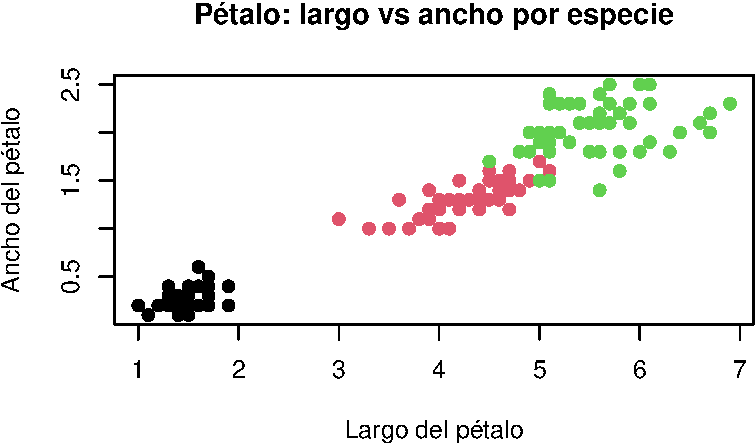
\includegraphics{sesion1_files/figure-pdf/unnamed-chunk-63-1.pdf}

\chapter{Paquetes}\label{paquetes}

En R, muchas de las cosas que queremos hacer se pueden realizar con
\emph{paquetes}. En R, un paquete es generalmente un conjunto de
herramientas con funciones específicas para realizar tareas específicas.
Para casi todo hay paquetes.

Por ejemplo, el paquete \texttt{dplyr} es un paquete ampliamente
utilizado para la manipulación de datos como filtrar valores o crear
nuevas columnas. Pero antes, necesitamos entender la diferencia entre
instalar un paquete y cargar un paquete en R.

\section{Instalar un paquete}\label{instalar-un-paquete}

Me gusta pensar que instalar un paquete en R es similar a ir a la tienda
y comprar una caja de herramientas. Después de comprarla, la mueves a tu
propio almacén para asegurarte de que la tendrás cuando la necesites.
Esto solo necesita hacerse una vez por paquete, a menos que quieras
actualizarlo (tener la última versión).

Con R, instalamos un paquete con una función llamada
\texttt{install.packages()} seguida del nombre del paquete entre
comillas.

\begin{Shaded}
\begin{Highlighting}[]
\FunctionTok{install.packages}\NormalTok{(}\StringTok{\textquotesingle{}dplyr\textquotesingle{}}\NormalTok{)}
\end{Highlighting}
\end{Shaded}

\section{Cargar un paquete}\label{cargar-un-paquete}

Cuando cargas un paquete en R, es como si sacaras la caja de
herramientas del almacén y la pusieras en tu mesa de trabajo. Solo
entonces las herramientas dentro de la caja te son accesibles para tus
proyectos. Haces esto cada vez que comienzas un nuevo documento o una
sesión de R.

Para hacerlo, usamos la función \texttt{library()}.

\begin{Shaded}
\begin{Highlighting}[]
\FunctionTok{library}\NormalTok{(dplyr)}
\end{Highlighting}
\end{Shaded}

También puedes lograr esto con~\texttt{::}~si quieres usar una función
completa de otro paquete, pero no quieres cargar el paquete completo.
Esto es como sacar una herramienta específica de la caja, pero no poner
toda la caja en tu mesa de trabajo.

Por ejemplo, el paquete~\texttt{psych}~tiene una
función~\texttt{describe}~que produce un resumen estadístico detallado
de un conjunto de datos dado. Si queremos aplicarlo en un conjunto de
datos predeterminado en R como~\texttt{iris}, podemos hacerlo sin cargar
todo~\texttt{psych}:

\begin{Shaded}
\begin{Highlighting}[]
\NormalTok{psych}\SpecialCharTok{::}\FunctionTok{describe}\NormalTok{(iris)}
\end{Highlighting}
\end{Shaded}

Proporciona un resumen estadístico de los datos: media, desviación
estándar, mínimo, máximo, etc., todo sin tener que cargar todo el
paquete~\texttt{psych}.

\begin{verbatim}
               n mean   sd median min max   se
Sepal.Length 150 5.84 0.83   5.80 4.3 7.9 0.07
Sepal.Width  150 3.06 0.44   3.00 2.0 4.4 0.04
Petal.Length 150 3.76 1.77   4.35 1.0 6.9 0.14
Petal.Width  150 1.20 0.76   1.30 0.1 2.5 0.06
Species*     150 2.00 0.82   2.00 1.0 3.0 0.07
\end{verbatim}

\texttt{glimpse()} es una función de \texttt{dplyr} que proporciona una
vista compacta del dataframe, mostrando los nombres de las variables,
sus tipos de datos y una muestra de valores.

\begin{Shaded}
\begin{Highlighting}[]
\FunctionTok{glimpse}\NormalTok{(iris)}
\end{Highlighting}
\end{Shaded}

\begin{verbatim}
Rows: 150
Columns: 5
$ Sepal.Length <dbl> 5.1, 4.9, 4.7, 4.6, 5.0, 5.4, 4.6, 5.0, 4.4, 4.9, 5.4, 4.~
$ Sepal.Width  <dbl> 3.5, 3.0, 3.2, 3.1, 3.6, 3.9, 3.4, 3.4, 2.9, 3.1, 3.7, 3.~
$ Petal.Length <dbl> 1.4, 1.4, 1.3, 1.5, 1.4, 1.7, 1.4, 1.5, 1.4, 1.5, 1.5, 1.~
$ Petal.Width  <dbl> 0.2, 0.2, 0.2, 0.2, 0.2, 0.4, 0.3, 0.2, 0.2, 0.1, 0.2, 0.~
$ Species      <fct> setosa, setosa, setosa, setosa, setosa, setosa, setosa, s~
\end{verbatim}

\textbf{Recuerda:}

\begin{itemize}
\item
  Cuando \textbf{instalas un paquete}, estás tomando la caja de
  herramientas y asegurándola en tu propio almacén.
\item
  \textbf{Cargar un paquete}, entonces, es poner esa caja de
  herramientas en tu mesa de trabajo para que puedas usar sus
  herramientas.
\item
  \textbf{Importar una función del paquete} es como sacar una
  herramienta de la caja.
\end{itemize}

\chapter{Importación}\label{importaciuxf3n}

El primer paso al analizar datos generalmente conociste en
\textbf{importar los datos desde fuentes externas} al entorno de R. Por
ejemplo, en las ciencias sociales, los investigadores suelen trabajar
con bases de datos provenientes de encuestas, experimentos o datos
recolectados en plataformas como hojas de cálculo de Excel, herramientas
de encuestas en línea o programas de análisis estadístico como SPSS o
Stata.

\begin{tcolorbox}[enhanced jigsaw, titlerule=0mm, title=\textcolor{quarto-callout-note-color}{\faInfo}\hspace{0.5em}{Dato}, colback=white, opacityback=0, breakable, toprule=.15mm, left=2mm, leftrule=.75mm, colframe=quarto-callout-note-color-frame, bottomtitle=1mm, rightrule=.15mm, opacitybacktitle=0.6, coltitle=black, arc=.35mm, bottomrule=.15mm, toptitle=1mm, colbacktitle=quarto-callout-note-color!10!white]

Aunque R incluye funciones base (viene por defecto y no necesitan cargar
algún paquete) para la importación de datos, como~\texttt{read.csv()},
nos enfocaremos en los paquetes especializados
como~\textbf{\texttt{readr}},~\textbf{\texttt{readxl}}~y~\textbf{\texttt{haven}},
que son más actuales y generan~\textbf{\texttt{tibbles}}, una versión
mejorada de los \texttt{data.frames}.

\end{tcolorbox}

Los archivos que utilizaremos a lo largo de este libro están disponibles
en la~\textbf{carpeta de archivos del libro}, la cual se recomienda
descargar y guardar en una~\textbf{carpeta de trabajo}~en tu
computadora. Para seguir los ejemplos en este capítulo, asegúrate de
tener los archivos en tu carpeta de trabajo y configurar tu directorio
de trabajo en RStudio.

El formato~\textbf{CSV}~(Comma-Separated Values) es uno de los más
utilizados debido a su simplicidad y compatibilidad. Cada fila en un
archivo CSV representa una observación, y los valores dentro de cada
fila están separados por comas.

Un ejemplo de cómo podría lucir un archivo CSV:

\begin{verbatim}
ID,Edad,Género,Ingreso
1,25,Femenino,1500
2,30,Masculino,2000
3,45,Femenino,2500
\end{verbatim}

El paquete \textbf{\texttt{readr}} es parte del tidyverse y está
diseñado para leer archivos CSV.

\begin{Shaded}
\begin{Highlighting}[]
\CommentTok{\# Cargamos el paquete readr}
\FunctionTok{library}\NormalTok{(readr)}
\end{Highlighting}
\end{Shaded}

Al importar un conjunto de datos debemos nombrarlo.

\begin{Shaded}
\begin{Highlighting}[]
\CommentTok{\# Importamos el archivo CSV y lo asignamos a un objeto}
\NormalTok{encuesta\_csv }\OtherTok{=} \FunctionTok{read\_csv}\NormalTok{(}\StringTok{"encuesta.csv"}\NormalTok{)}
\NormalTok{encuesta\_csv}
\end{Highlighting}
\end{Shaded}

\begin{verbatim}
# A tibble: 8 x 3
  genero    medio_comunicación  edad
  <chr>     <chr>              <dbl>
1 Masculino Televisión            34
2 Femenino  Redes sociales        25
3 Femenino  Redes sociales        55
4 Otro      Radio                 63
5 Femenino  Televisión            47
6 Masculino Redes sociales        19
# i 2 more rows
\end{verbatim}

Los archivos de Excel son comunes en las ciencias sociales debido a su
facilidad de uso y capacidad para almacenar datos tabulares en varias
hojas. El paquete \textbf{\texttt{readxl}} permite importar estos
archivos, ya sea en formato~\texttt{.xls}~o~\texttt{.xlsx}, sin
necesidad de tener Excel instalado.

\begin{Shaded}
\begin{Highlighting}[]
\CommentTok{\# Cargamos el paquete readxl}
\FunctionTok{library}\NormalTok{(readxl)}
\end{Highlighting}
\end{Shaded}

\begin{Shaded}
\begin{Highlighting}[]
\CommentTok{\# Importamos los datos desde un archivo Excel}
\NormalTok{encuesta\_excel }\OtherTok{=} \FunctionTok{read\_excel}\NormalTok{(}\StringTok{"encuesta.xlsx"}\NormalTok{)}
\NormalTok{encuesta\_excel}
\end{Highlighting}
\end{Shaded}

\begin{verbatim}
# A tibble: 10 x 3
  genero    medio_comunicación  edad
  <chr>     <chr>              <dbl>
1 Masculino Televisión            34
2 Femenino  Redes sociales        NA
3 Femenino  Redes sociales        55
4 Otro      Radio                 63
5 Femenino  Televisión            NA
6 Masculino Redes sociales        19
# i 4 more rows
\end{verbatim}

Si el archivo contiene múltiples hojas, podemos especificar cuál
importar utilizando el argumento~\texttt{sheet}:

\begin{Shaded}
\begin{Highlighting}[]
\NormalTok{encuesta\_excel\_hoja }\OtherTok{=} \FunctionTok{read\_excel}\NormalTok{(}\StringTok{"encuesta.xlsx"}\NormalTok{, }
                                  \AttributeTok{sheet =} \StringTok{"Resultados"}\NormalTok{)}
\end{Highlighting}
\end{Shaded}

\chapter{Limpieza}\label{limpieza}

Una vez que hemos importado los datos, el siguiente paso es limpiarlos.
Este proceso consiste en identificar y corregir problemas comunes como
valores faltantes, nombres de columnas inconsistentes, duplicados y
tipos de datos incorrectos. La limpieza asegura que los datos estén en
un estado coherente y listo para ser transformado o analizado.

\section{Manejo de valores faltantes}\label{manejo-de-valores-faltantes}

El \textbf{manejo de valores faltantes} es uno de los aspectos más
complejos en la limpieza de datos, y un tema importante a considerar al
trabajar con conjuntos de datos. Un \textbf{valor perdido} o \textbf{NA}
en R no es lo mismo que un \textbf{0} o un espacio vacío. Un valor
perdido (o \textbf{NA}, que significa ``Not Available'') es una celda
que no contiene información en absoluto, lo que puede ocurrir por
diversas razones, como un error en la recolección de los datos, una
respuesta no proporcionada en una encuesta o una omisión involuntaria al
momento de ingresar los datos.

Por ejemplo:

\begin{Shaded}
\begin{Highlighting}[]
\NormalTok{encuesta\_excel}
\end{Highlighting}
\end{Shaded}

\begin{verbatim}
# A tibble: 10 x 3
  genero    medio_comunicación  edad
  <chr>     <chr>              <dbl>
1 Masculino Televisión            34
2 Femenino  Redes sociales        NA
3 Femenino  Redes sociales        55
4 Otro      Radio                 63
5 Femenino  Televisión            NA
6 Masculino Redes sociales        19
# i 4 more rows
\end{verbatim}

Puedes detectar estos valores la función como \texttt{is.na()}, que
devuelve un valor lógico (\texttt{TRUE} o \texttt{FALSE}) indicando si
un valor es \texttt{NA}. Seleccionamos la columna.

\begin{Shaded}
\begin{Highlighting}[]
\FunctionTok{is.na}\NormalTok{(encuesta\_excel}\SpecialCharTok{$}\NormalTok{edad)}
\end{Highlighting}
\end{Shaded}

\begin{verbatim}
 [1] FALSE  TRUE FALSE FALSE  TRUE FALSE FALSE FALSE FALSE FALSE
\end{verbatim}

Recuerda que puedes sumar un vector lógico para contar los TRUE. En este
caso los valores perdidos.

\begin{Shaded}
\begin{Highlighting}[]
\CommentTok{\# Cantidad de valores perdidos }
\FunctionTok{sum}\NormalTok{(}\FunctionTok{is.na}\NormalTok{(encuesta\_excel}\SpecialCharTok{$}\NormalTok{edad)) }
\end{Highlighting}
\end{Shaded}

\begin{verbatim}
[1] 2
\end{verbatim}

Una de las formas más simples de manejar valores faltantes es
eliminarlos por completo. Esto puede hacerse utilizando la
función~\texttt{drop\_na()}~del paquete~\texttt{tidyr}, que elimina las
filas que contienen al menos un valor NA en cualquier columna. Esta es
una solución rápida, pero es importante ser cauteloso, ya que puede
resultar en la pérdida de información valiosa si hay muchos datos
faltantes.

\begin{Shaded}
\begin{Highlighting}[]
\CommentTok{\# Cargamos tidyr}
\FunctionTok{library}\NormalTok{(tidyr)}
\end{Highlighting}
\end{Shaded}

\begin{Shaded}
\begin{Highlighting}[]
\CommentTok{\# Eliminamos filas con valores faltantes}
\FunctionTok{drop\_na}\NormalTok{(encuesta\_excel)}
\end{Highlighting}
\end{Shaded}

\begin{verbatim}
# A tibble: 7 x 3
  genero    medio_comunicación  edad
  <chr>     <chr>              <dbl>
1 Masculino Televisión            34
2 Femenino  Redes sociales        55
3 Otro      Radio                 63
4 Masculino Redes sociales        19
5 Masculino Periódico             75
6 Femenino  Redes sociales        55
# i 1 more row
\end{verbatim}

Comparemos

\begin{Shaded}
\begin{Highlighting}[]
\CommentTok{\# Podemos nombrarlo}
\NormalTok{encuesta\_sin\_na }\OtherTok{=} \FunctionTok{drop\_na}\NormalTok{(encuesta\_excel)}
\end{Highlighting}
\end{Shaded}

Presta atención a las dimensiones del tibble original y del tibble sin
\texttt{NA}

\begin{Shaded}
\begin{Highlighting}[]
\FunctionTok{dim}\NormalTok{(encuesta\_excel)}
\end{Highlighting}
\end{Shaded}

\begin{verbatim}
[1] 10  3
\end{verbatim}

\begin{Shaded}
\begin{Highlighting}[]
\FunctionTok{dim}\NormalTok{(encuesta\_sin\_na)}
\end{Highlighting}
\end{Shaded}

\begin{verbatim}
[1] 7 3
\end{verbatim}

Si queremos ser más específicos y eliminar valores faltantes solo en una
columna particular, podemos usar:

\begin{Shaded}
\begin{Highlighting}[]
\CommentTok{\# Eliminamos filas donde la columna \textquotesingle{}edad\textquotesingle{} tiene NA}
\NormalTok{encuesta\_sin\_na }\OtherTok{=} \FunctionTok{drop\_na}\NormalTok{(encuesta\_excel, edad)}

\NormalTok{encuesta\_sin\_na}
\end{Highlighting}
\end{Shaded}

\begin{verbatim}
# A tibble: 8 x 3
  genero    medio_comunicación  edad
  <chr>     <chr>              <dbl>
1 Masculino Televisión            34
2 Femenino  Redes sociales        55
3 Otro      Radio                 63
4 Masculino Redes sociales        19
5 Masculino <NA>                  29
6 Masculino Periódico             75
# i 2 more rows
\end{verbatim}

\begin{tcolorbox}[enhanced jigsaw, titlerule=0mm, title=\textcolor{quarto-callout-caution-color}{\faFire}\hspace{0.5em}{Cuidado}, colback=white, opacityback=0, breakable, toprule=.15mm, left=2mm, leftrule=.75mm, colframe=quarto-callout-caution-color-frame, bottomtitle=1mm, rightrule=.15mm, opacitybacktitle=0.6, coltitle=black, arc=.35mm, bottomrule=.15mm, toptitle=1mm, colbacktitle=quarto-callout-caution-color!10!white]

Aunque eliminar valores faltantes puede ser un enfoque válido en algunos
casos, \textbf{no siempre es ideal}. Si eliminamos demasiadas filas,
podemos perder una cantidad significativa de información, lo que podría
alterar los resultados de nuestro análisis. Por eso, en lugar de
eliminar, muchas veces es preferible \textbf{imputar los valores
faltantes}, es decir, reemplazarlos con un valor estimado. Por ejemplo,
algunas estrategias comunes para imputar valores incluyen
\textbf{reemplazar por el promedio} en el caso de variables numéricas o
\textbf{reemplazar por la moda} en variables categóricas donde los
valores faltantes pueden ser reemplazados por el valor más frecuente (la
moda).

\end{tcolorbox}

Para las siguentes técnicas de limpieza utilizaremos el conjunto de
datos \texttt{encuesta\_problematica}. Te animo a que puedas identificar
que posible problemas tiene antes de seguir adelante.

\begin{Shaded}
\begin{Highlighting}[]
\NormalTok{datos\_problema }\OtherTok{=} \FunctionTok{read.csv}\NormalTok{(}\StringTok{\textquotesingle{}encuesta\_problematica.csv\textquotesingle{}}\NormalTok{)}

\NormalTok{datos\_problema}
\end{Highlighting}
\end{Shaded}

\begin{verbatim}
  ID Nombre.PARTICIPANTE EDAD..años. Ingreso.Mensual género
1  1         Luis Bartra          23            1500      F
2  2        Carlos Gómez          27            2000      M
3  2        Carlos Gómez          27            2000      M
4  3         María López          45            2500      F
5  4       Javier Muller          35            3800      M
6  5          Liz García          29            1800      M
\end{verbatim}

\section{Estandarización de nombres de
columnas}\label{estandarizaciuxf3n-de-nombres-de-columnas}

Los nombres de las columnas en los conjuntos de datos pueden ser
inconsistentes, incluir caracteres especiales o espacios que dificulten
el manejo en R.

Primero, identificamos los nombres originales del conjunto de datos
utilizando la función base names():

\begin{Shaded}
\begin{Highlighting}[]
\FunctionTok{colnames}\NormalTok{(datos\_problema)}
\end{Highlighting}
\end{Shaded}

\begin{verbatim}
[1] "ID"                  "Nombre.PARTICIPANTE" "EDAD..años."        
[4] "Ingreso.Mensual"     "género"             
\end{verbatim}

Para resolver esto, utilizamos la función \texttt{clean\_names()} del
paquete \texttt{janitor}. Esta función transforma automáticamente los
nombres de las columnas en un formato limpio y consistente:

\begin{Shaded}
\begin{Highlighting}[]
\CommentTok{\# Cargar el paquete janitor}
\FunctionTok{library}\NormalTok{(janitor)}

\CommentTok{\# Estandarizar los nombres de las columnas}
\NormalTok{datos\_problema }\OtherTok{=} \FunctionTok{clean\_names}\NormalTok{(datos\_problema)}
\end{Highlighting}
\end{Shaded}

\begin{Shaded}
\begin{Highlighting}[]
\FunctionTok{colnames}\NormalTok{(datos\_problema)}
\end{Highlighting}
\end{Shaded}

\begin{verbatim}
[1] "id"                  "nombre_participante" "edad_anos"          
[4] "ingreso_mensual"     "genero"             
\end{verbatim}

\begin{Shaded}
\begin{Highlighting}[]
\FunctionTok{head}\NormalTok{(datos\_problema, }\DecValTok{3}\NormalTok{)}
\end{Highlighting}
\end{Shaded}

\begin{verbatim}
  id nombre_participante edad_anos ingreso_mensual genero
1  1         Luis Bartra        23            1500      F
2  2        Carlos Gómez        27            2000      M
3  2        Carlos Gómez        27            2000      M
\end{verbatim}

\section{Eliminación de duplicados}\label{eliminaciuxf3n-de-duplicados}

En algunos casos, los datos pueden contener filas duplicadas que
distorsionan el análisis. Podemos identificar y eliminar estas filas
utilizando la función \texttt{distinct()} de \texttt{dplyr}.

\begin{Shaded}
\begin{Highlighting}[]
\CommentTok{\# Vemos el problema}
\NormalTok{datos\_problema}
\end{Highlighting}
\end{Shaded}

\begin{verbatim}
  id nombre_participante edad_anos ingreso_mensual genero
1  1         Luis Bartra        23            1500      F
2  2        Carlos Gómez        27            2000      M
3  2        Carlos Gómez        27            2000      M
4  3         María López        45            2500      F
5  4       Javier Muller        35            3800      M
6  5          Liz García        29            1800      M
\end{verbatim}

\begin{Shaded}
\begin{Highlighting}[]
\CommentTok{\# Eliminamos filas duplicadas}
\NormalTok{datos\_limpios }\OtherTok{=} \FunctionTok{distinct}\NormalTok{(datos\_problema)}
\end{Highlighting}
\end{Shaded}

\begin{Shaded}
\begin{Highlighting}[]
\FunctionTok{nrow}\NormalTok{(datos\_problema)     }\CommentTok{\# Antes: 7 filas}
\end{Highlighting}
\end{Shaded}

\begin{verbatim}
[1] 6
\end{verbatim}

\begin{Shaded}
\begin{Highlighting}[]
\FunctionTok{nrow}\NormalTok{(datos\_limpios) }
\end{Highlighting}
\end{Shaded}

\begin{verbatim}
[1] 5
\end{verbatim}

Mostramos:

\begin{Shaded}
\begin{Highlighting}[]
\NormalTok{datos\_limpios}
\end{Highlighting}
\end{Shaded}

\begin{verbatim}
  id nombre_participante edad_anos ingreso_mensual genero
1  1         Luis Bartra        23            1500      F
2  2        Carlos Gómez        27            2000      M
3  3         María López        45            2500      F
4  4       Javier Muller        35            3800      M
5  5          Liz García        29            1800      M
\end{verbatim}

\chapter{Guardado y exportación de objetos de
trabajo}\label{guardado-y-exportaciuxf3n-de-objetos-de-trabajo}

Una vez que hemos creado, limpiado o transformado nuestros datos, es
importante \textbf{guardar} el resultado para no perder el trabajo
realizado. R permite guardar objetos de trabajo en distintos formatos,
tanto para \textbf{volver a usarlos dentro de R} como para
\textbf{compartirlos con otras personas} (por ejemplo, en formato Excel
o CSV).

\section{\texorpdfstring{Guardar como archivo
\texttt{.RDS}}{Guardar como archivo .RDS}}\label{guardar-como-archivo-.rds}

El formato \texttt{.RDS} es propio de R. Guarda \textbf{un solo objeto},
como un \texttt{data.frame}, conservando su estructura interna.

\begin{Shaded}
\begin{Highlighting}[]
\FunctionTok{saveRDS}\NormalTok{(datos\_limpios, }\AttributeTok{file =} \StringTok{"datos\_limpios.rds"}\NormalTok{)}
\end{Highlighting}
\end{Shaded}

Luego, puedes volver a cargarlo con:

\begin{Shaded}
\begin{Highlighting}[]
\NormalTok{datos\_limpios }\OtherTok{=} \FunctionTok{readRDS}\NormalTok{(}\StringTok{"datos\_limpios.rds"}\NormalTok{)}
\end{Highlighting}
\end{Shaded}

\begin{tcolorbox}[enhanced jigsaw, titlerule=0mm, title=\textcolor{quarto-callout-note-color}{\faInfo}\hspace{0.5em}{Dato}, colback=white, opacityback=0, breakable, toprule=.15mm, left=2mm, leftrule=.75mm, colframe=quarto-callout-note-color-frame, bottomtitle=1mm, rightrule=.15mm, opacitybacktitle=0.6, coltitle=black, arc=.35mm, bottomrule=.15mm, toptitle=1mm, colbacktitle=quarto-callout-note-color!10!white]

Esto es ideal cuando trabajas con datos procesados dentro de R y quieres
retomarlos luego \textbf{sin tener que rehacer todo el procesamiento}.

\end{tcolorbox}

\section{\texorpdfstring{Exportar como archivo
\texttt{.csv}}{Exportar como archivo .csv}}\label{exportar-como-archivo-.csv}

Para compartir o abrir en Excel u otros programas, lo más común es
exportar a CSV.

\begin{Shaded}
\begin{Highlighting}[]
\FunctionTok{write.csv}\NormalTok{(datos\_limpios, }
          \AttributeTok{file =} \StringTok{"datos\_limpios.csv"}\NormalTok{, }
          \AttributeTok{row.names =} \ConstantTok{FALSE}\NormalTok{)}
\end{Highlighting}
\end{Shaded}

\begin{itemize}
\tightlist
\item
  \texttt{row.names\ =\ FALSE} evita que R agregue una columna extra con
  los números de fila.
\end{itemize}

\section{Guardar todo el entorno de
trabajo}\label{guardar-todo-el-entorno-de-trabajo}

Si deseas guardar \textbf{todos los objetos que tienes cargados} en tu
sesión (variables, data frames, modelos, etc.):

\begin{Shaded}
\begin{Highlighting}[]
\FunctionTok{save.image}\NormalTok{(}\AttributeTok{file =} \StringTok{"mi\_entorno.RData"}\NormalTok{)}
\end{Highlighting}
\end{Shaded}

Y para volver a cargarlo en otra sesión de R:

\begin{Shaded}
\begin{Highlighting}[]
\FunctionTok{load}\NormalTok{(}\StringTok{"mi\_entorno.RData"}\NormalTok{)}
\end{Highlighting}
\end{Shaded}

\begin{tcolorbox}[enhanced jigsaw, titlerule=0mm, title=\textcolor{quarto-callout-important-color}{\faExclamation}\hspace{0.5em}{Importante}, colback=white, opacityback=0, breakable, toprule=.15mm, left=2mm, leftrule=.75mm, colframe=quarto-callout-important-color-frame, bottomtitle=1mm, rightrule=.15mm, opacitybacktitle=0.6, coltitle=black, arc=.35mm, bottomrule=.15mm, toptitle=1mm, colbacktitle=quarto-callout-important-color!10!white]

Es buena práctica guardar tus objetos \textbf{con nombres claros} y
organizarlos en carpetas por cada proyecto a realizar. Esto no solo
garantiza el orden entre disntintos proyectos, sino que mejora la
reproducibilidad y facilita compartir tu análisis con otras personas o
retomarlo en el futuro.

\end{tcolorbox}




\end{document}
